\section*{Point P$_\mathbf{8}$($o_1=0{,}8 \, \mathrm{ cm}$)}
\begin{figure}[H]
	
	\subsection*{Mean velocities}
	\vspace{-3mm}
	\rule{\textwidth}{0.4pt}
	
	\begin{subfigure}{0.60\textwidth}
		\centering
		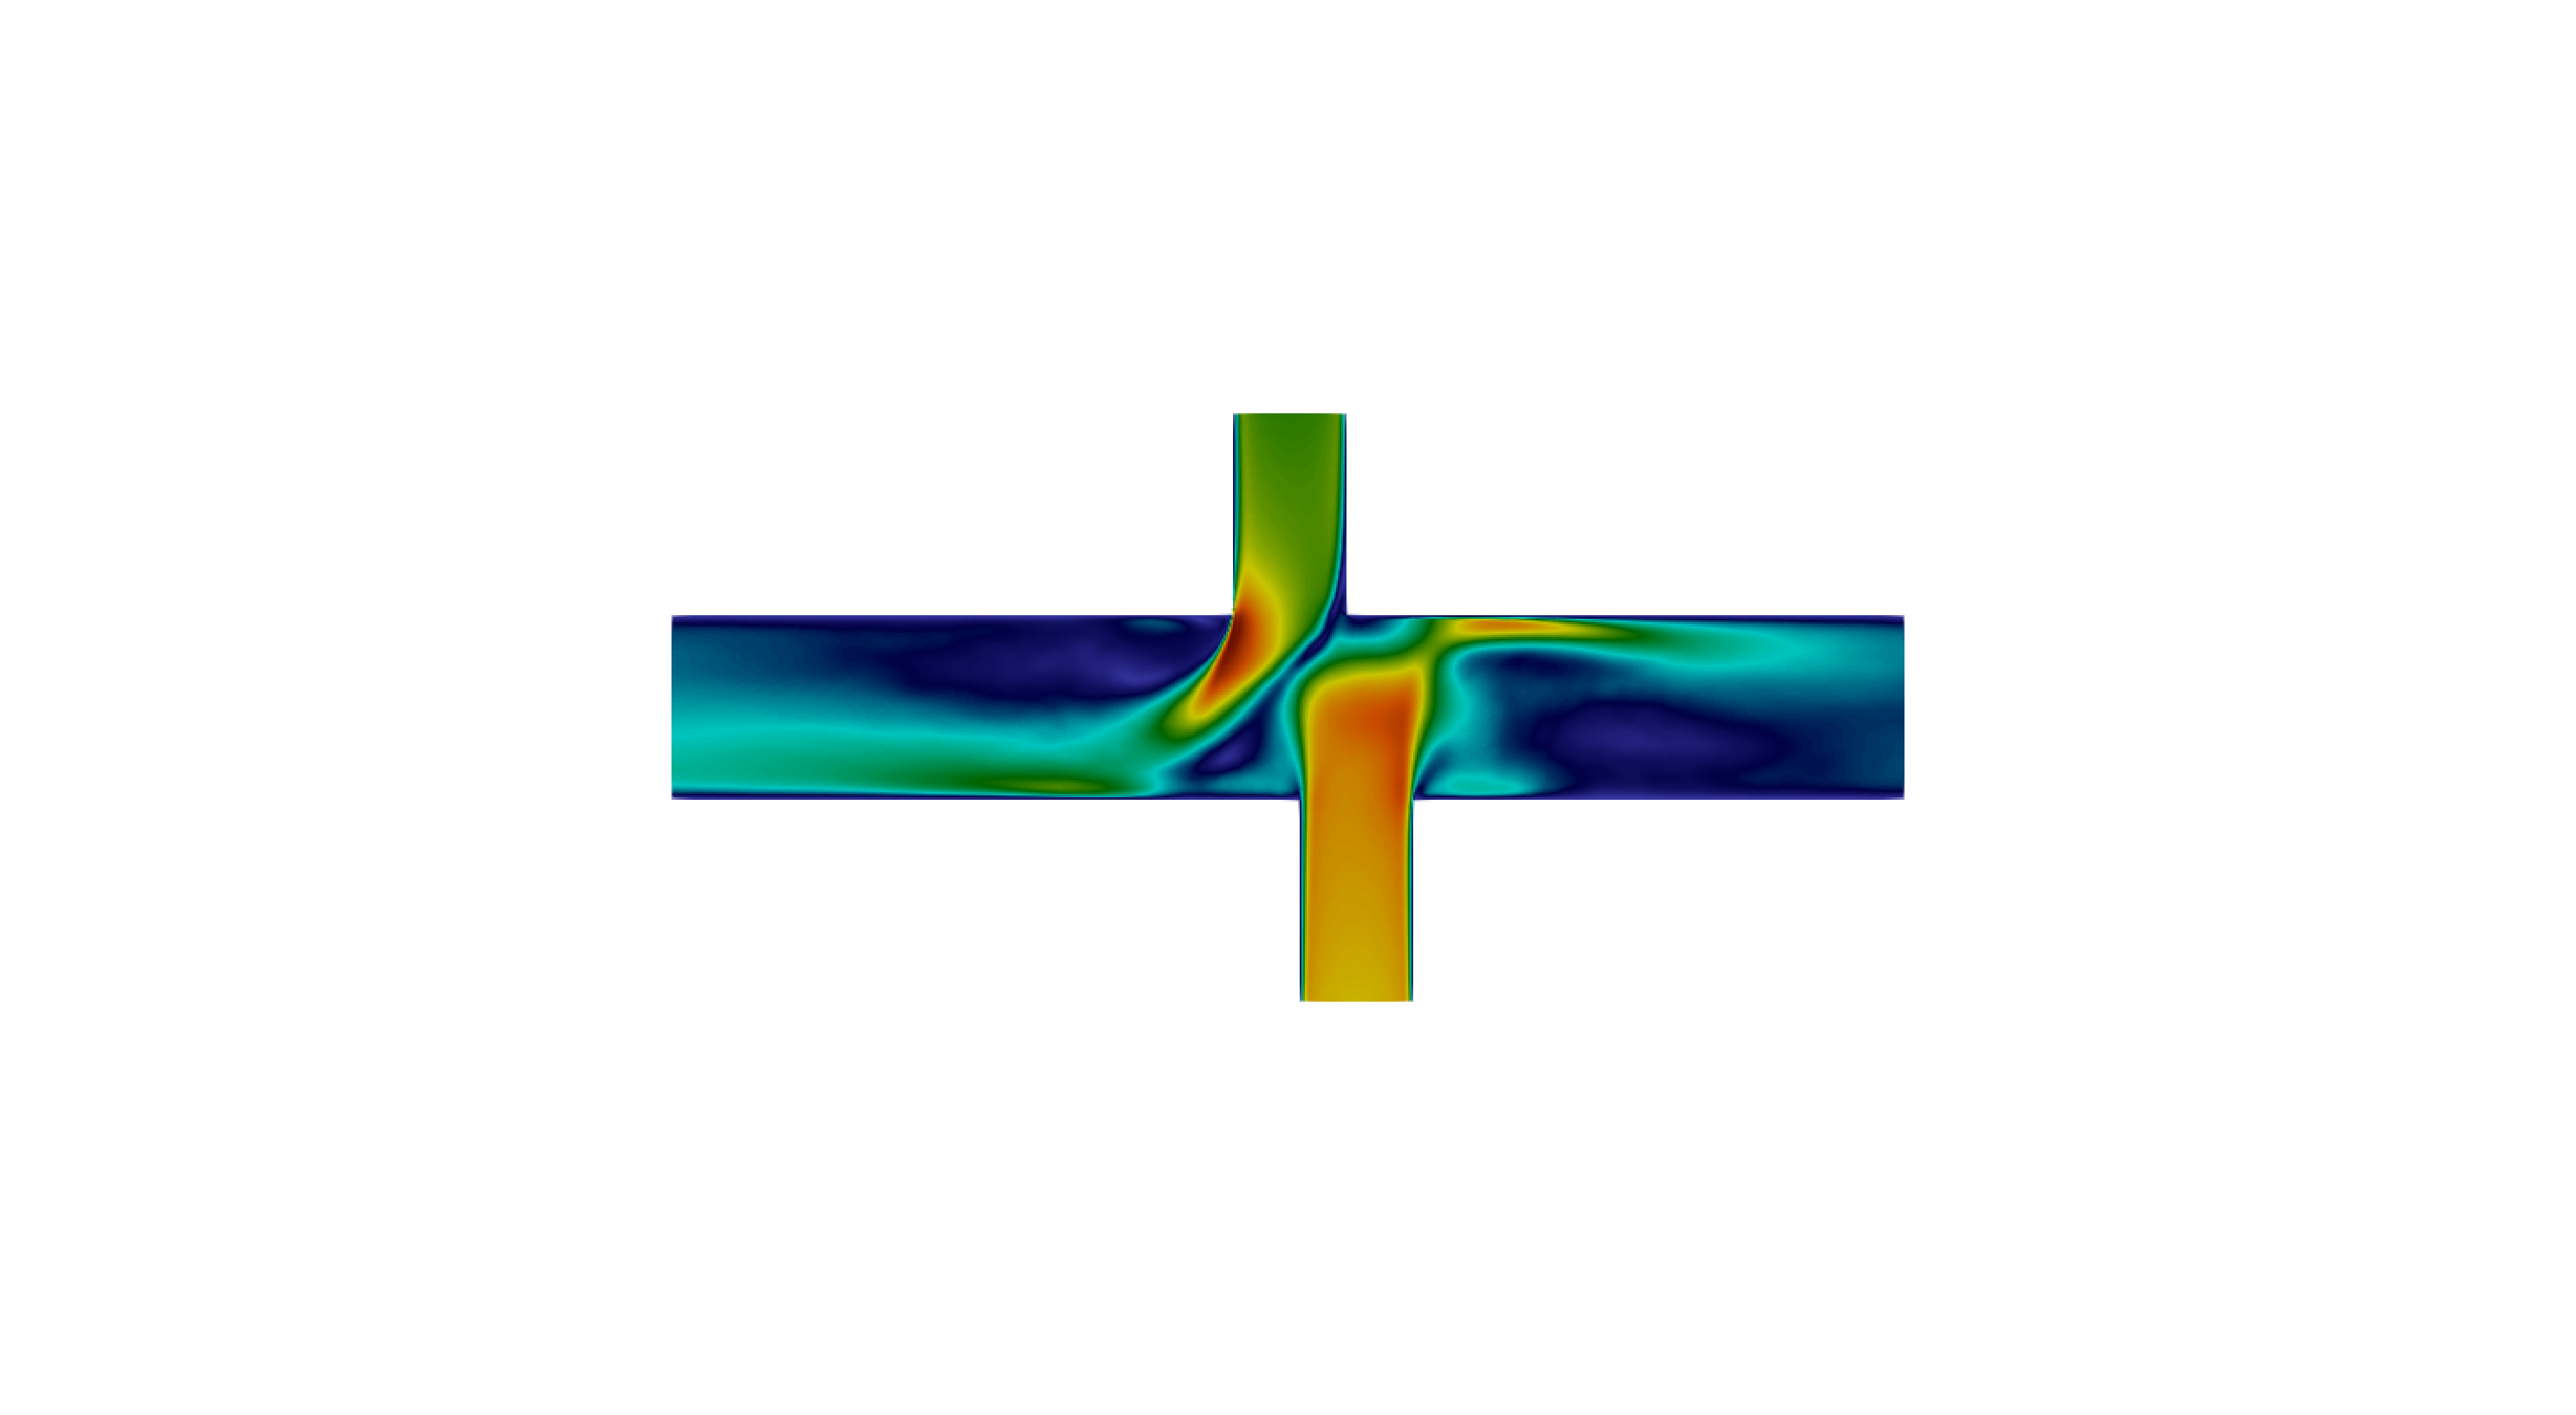
\includegraphics[
		width=\textwidth,
		trim={130mm 70mm 130mm 70mm},
		clip
		]
		{figures/plots/08/08_mean_veloc_xz.pdf}%
		\rlap{\hspace{-9.5cm}\raisebox{-0.0cm}{%  move next graphics to top right corner
				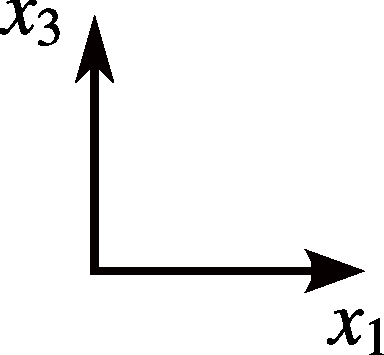
\includegraphics[height=1.5cm]{figures/x1x3.pdf}%
		}}
		
		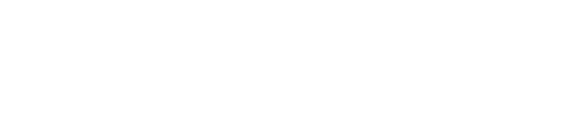
\includegraphics[
		width=0.85\textwidth,
		]
		{figures/plots/filler.pdf}
		\caption{Mean velocity magnitude field in the \(x_1\)-\(x_3\) plane.}
		\label{fig:mean_velocity_xz08}
		
	\end{subfigure}\hfill%
	\begin{subfigure}{0.36\textwidth}
		\vspace{14mm}
		\centering
		LPA\hspace{24mm}RPA
		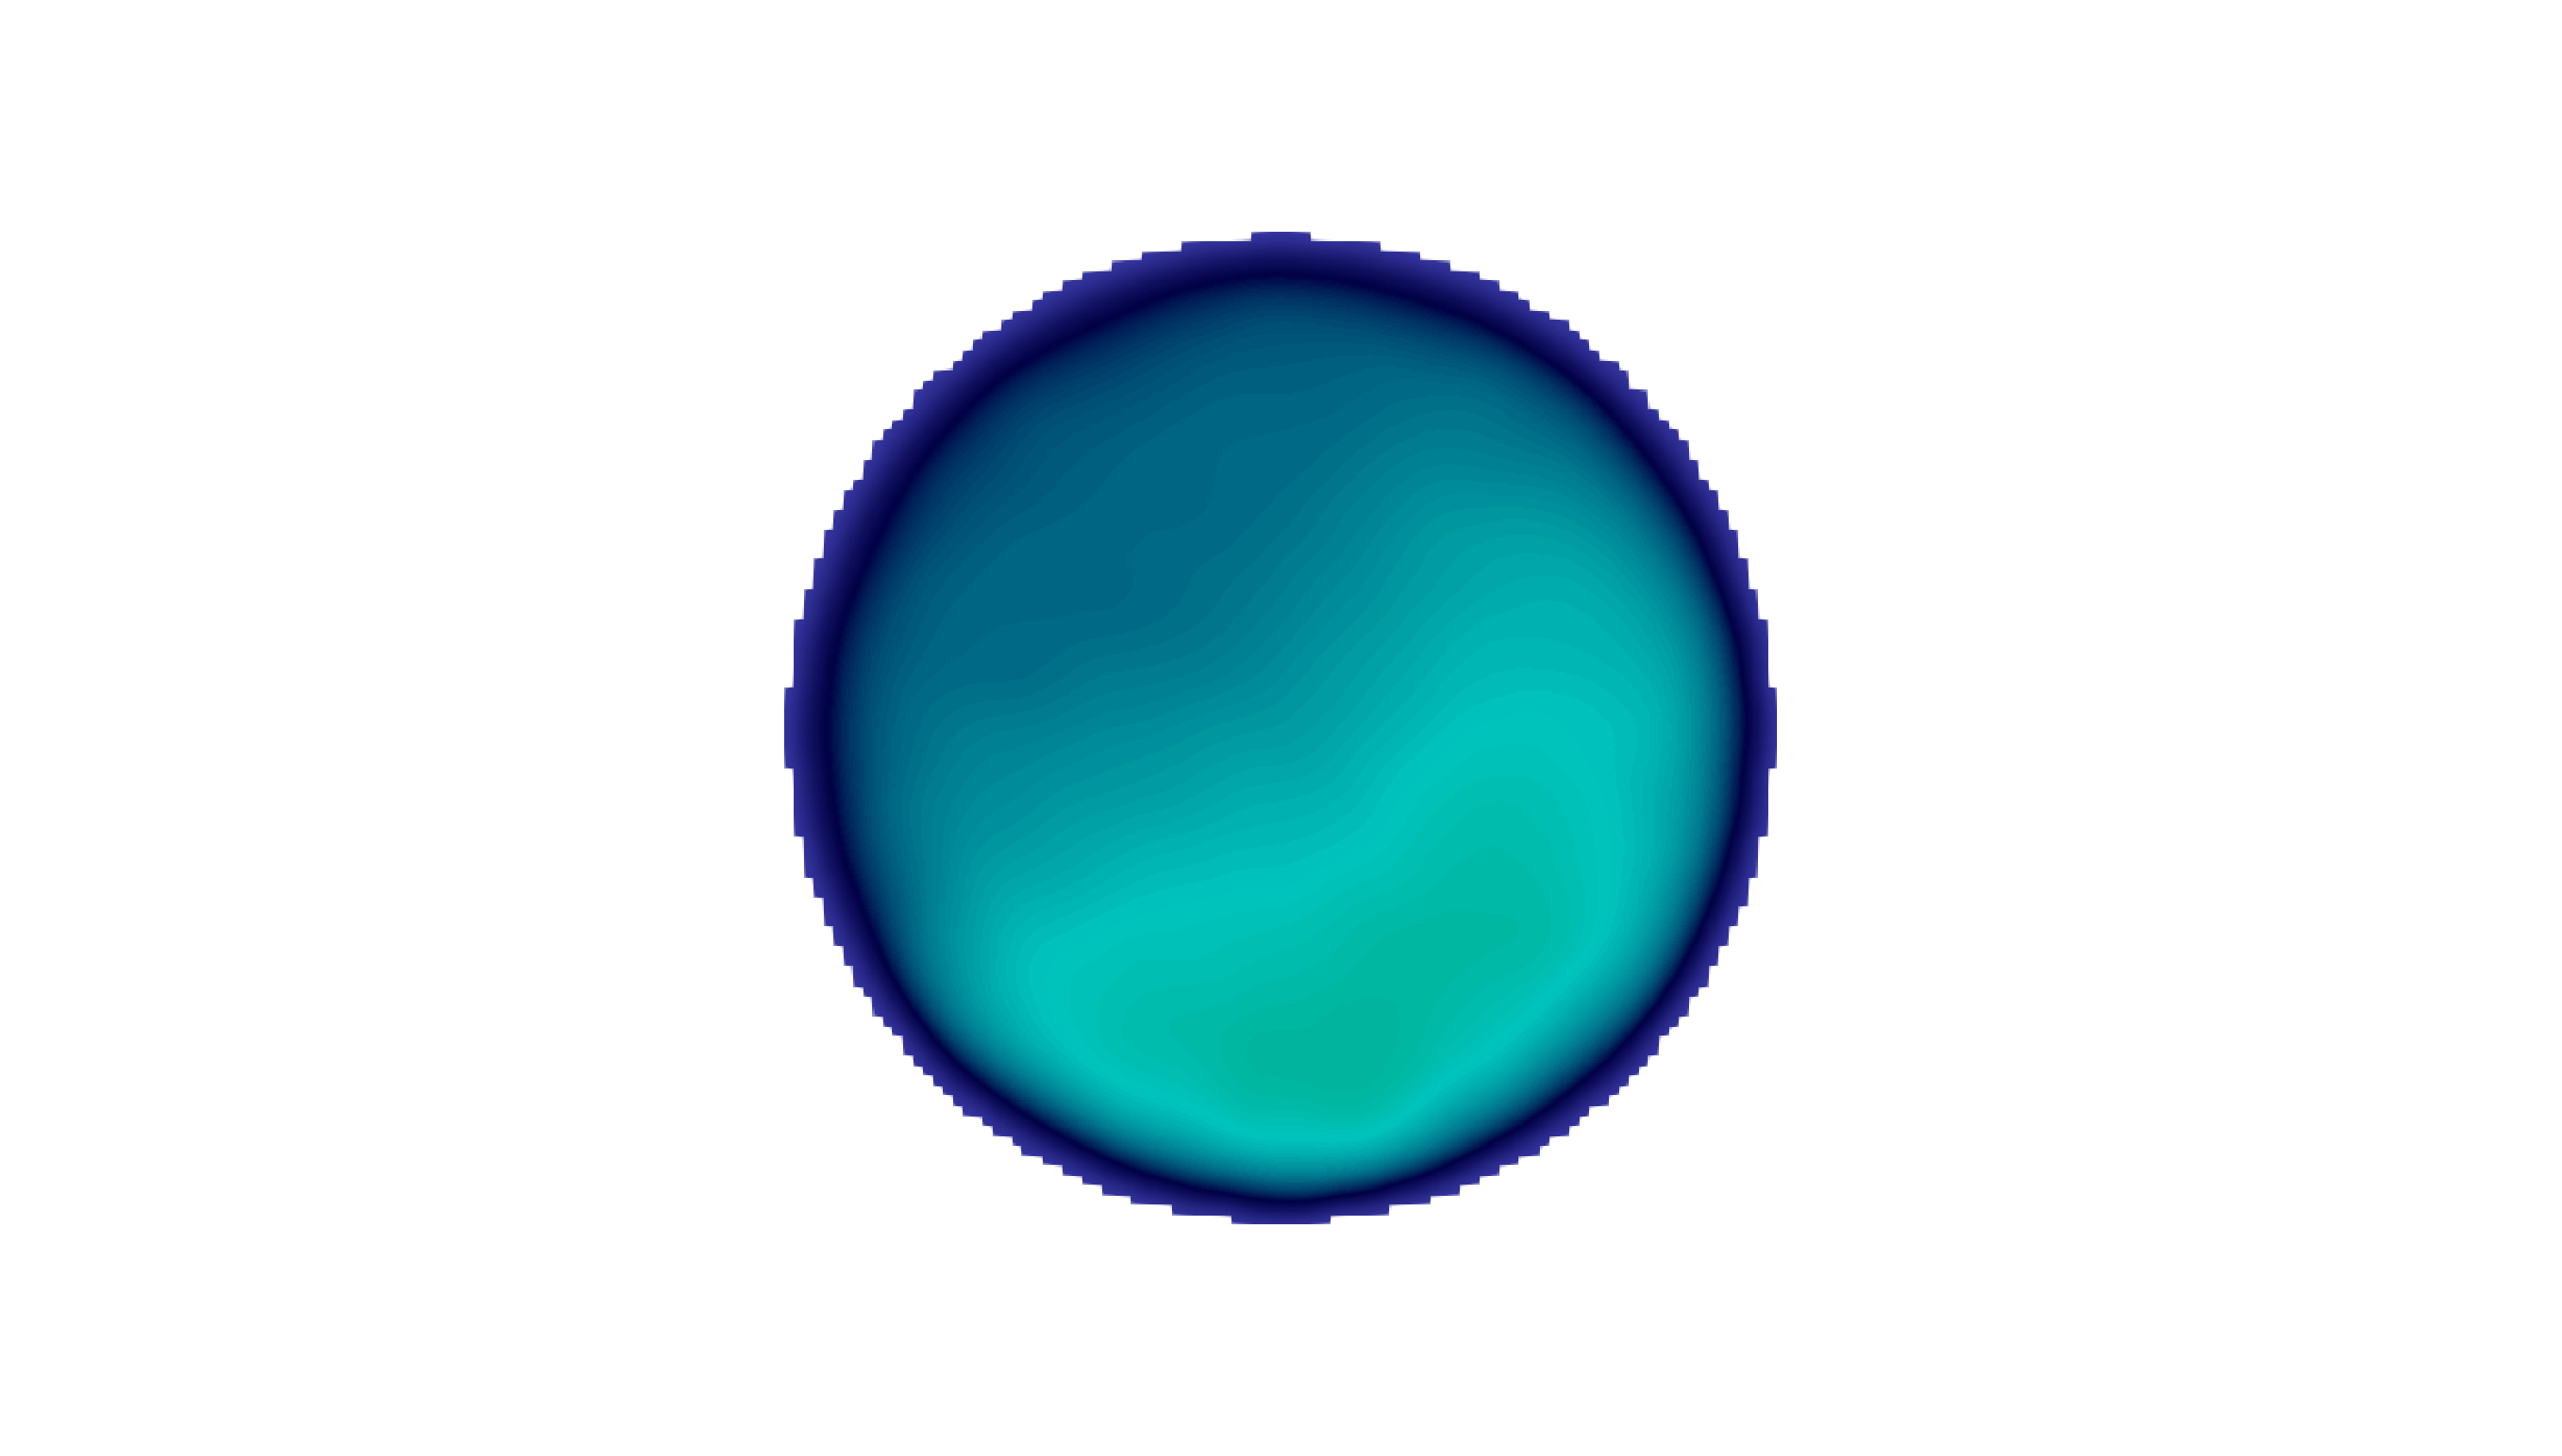
\includegraphics[
		width=0.46\textwidth,
		trim={150mm 20mm 150mm 20mm},
		clip
		]
		{figures/plots/08/08_LPA_mean_veloc.pdf}\hfill
		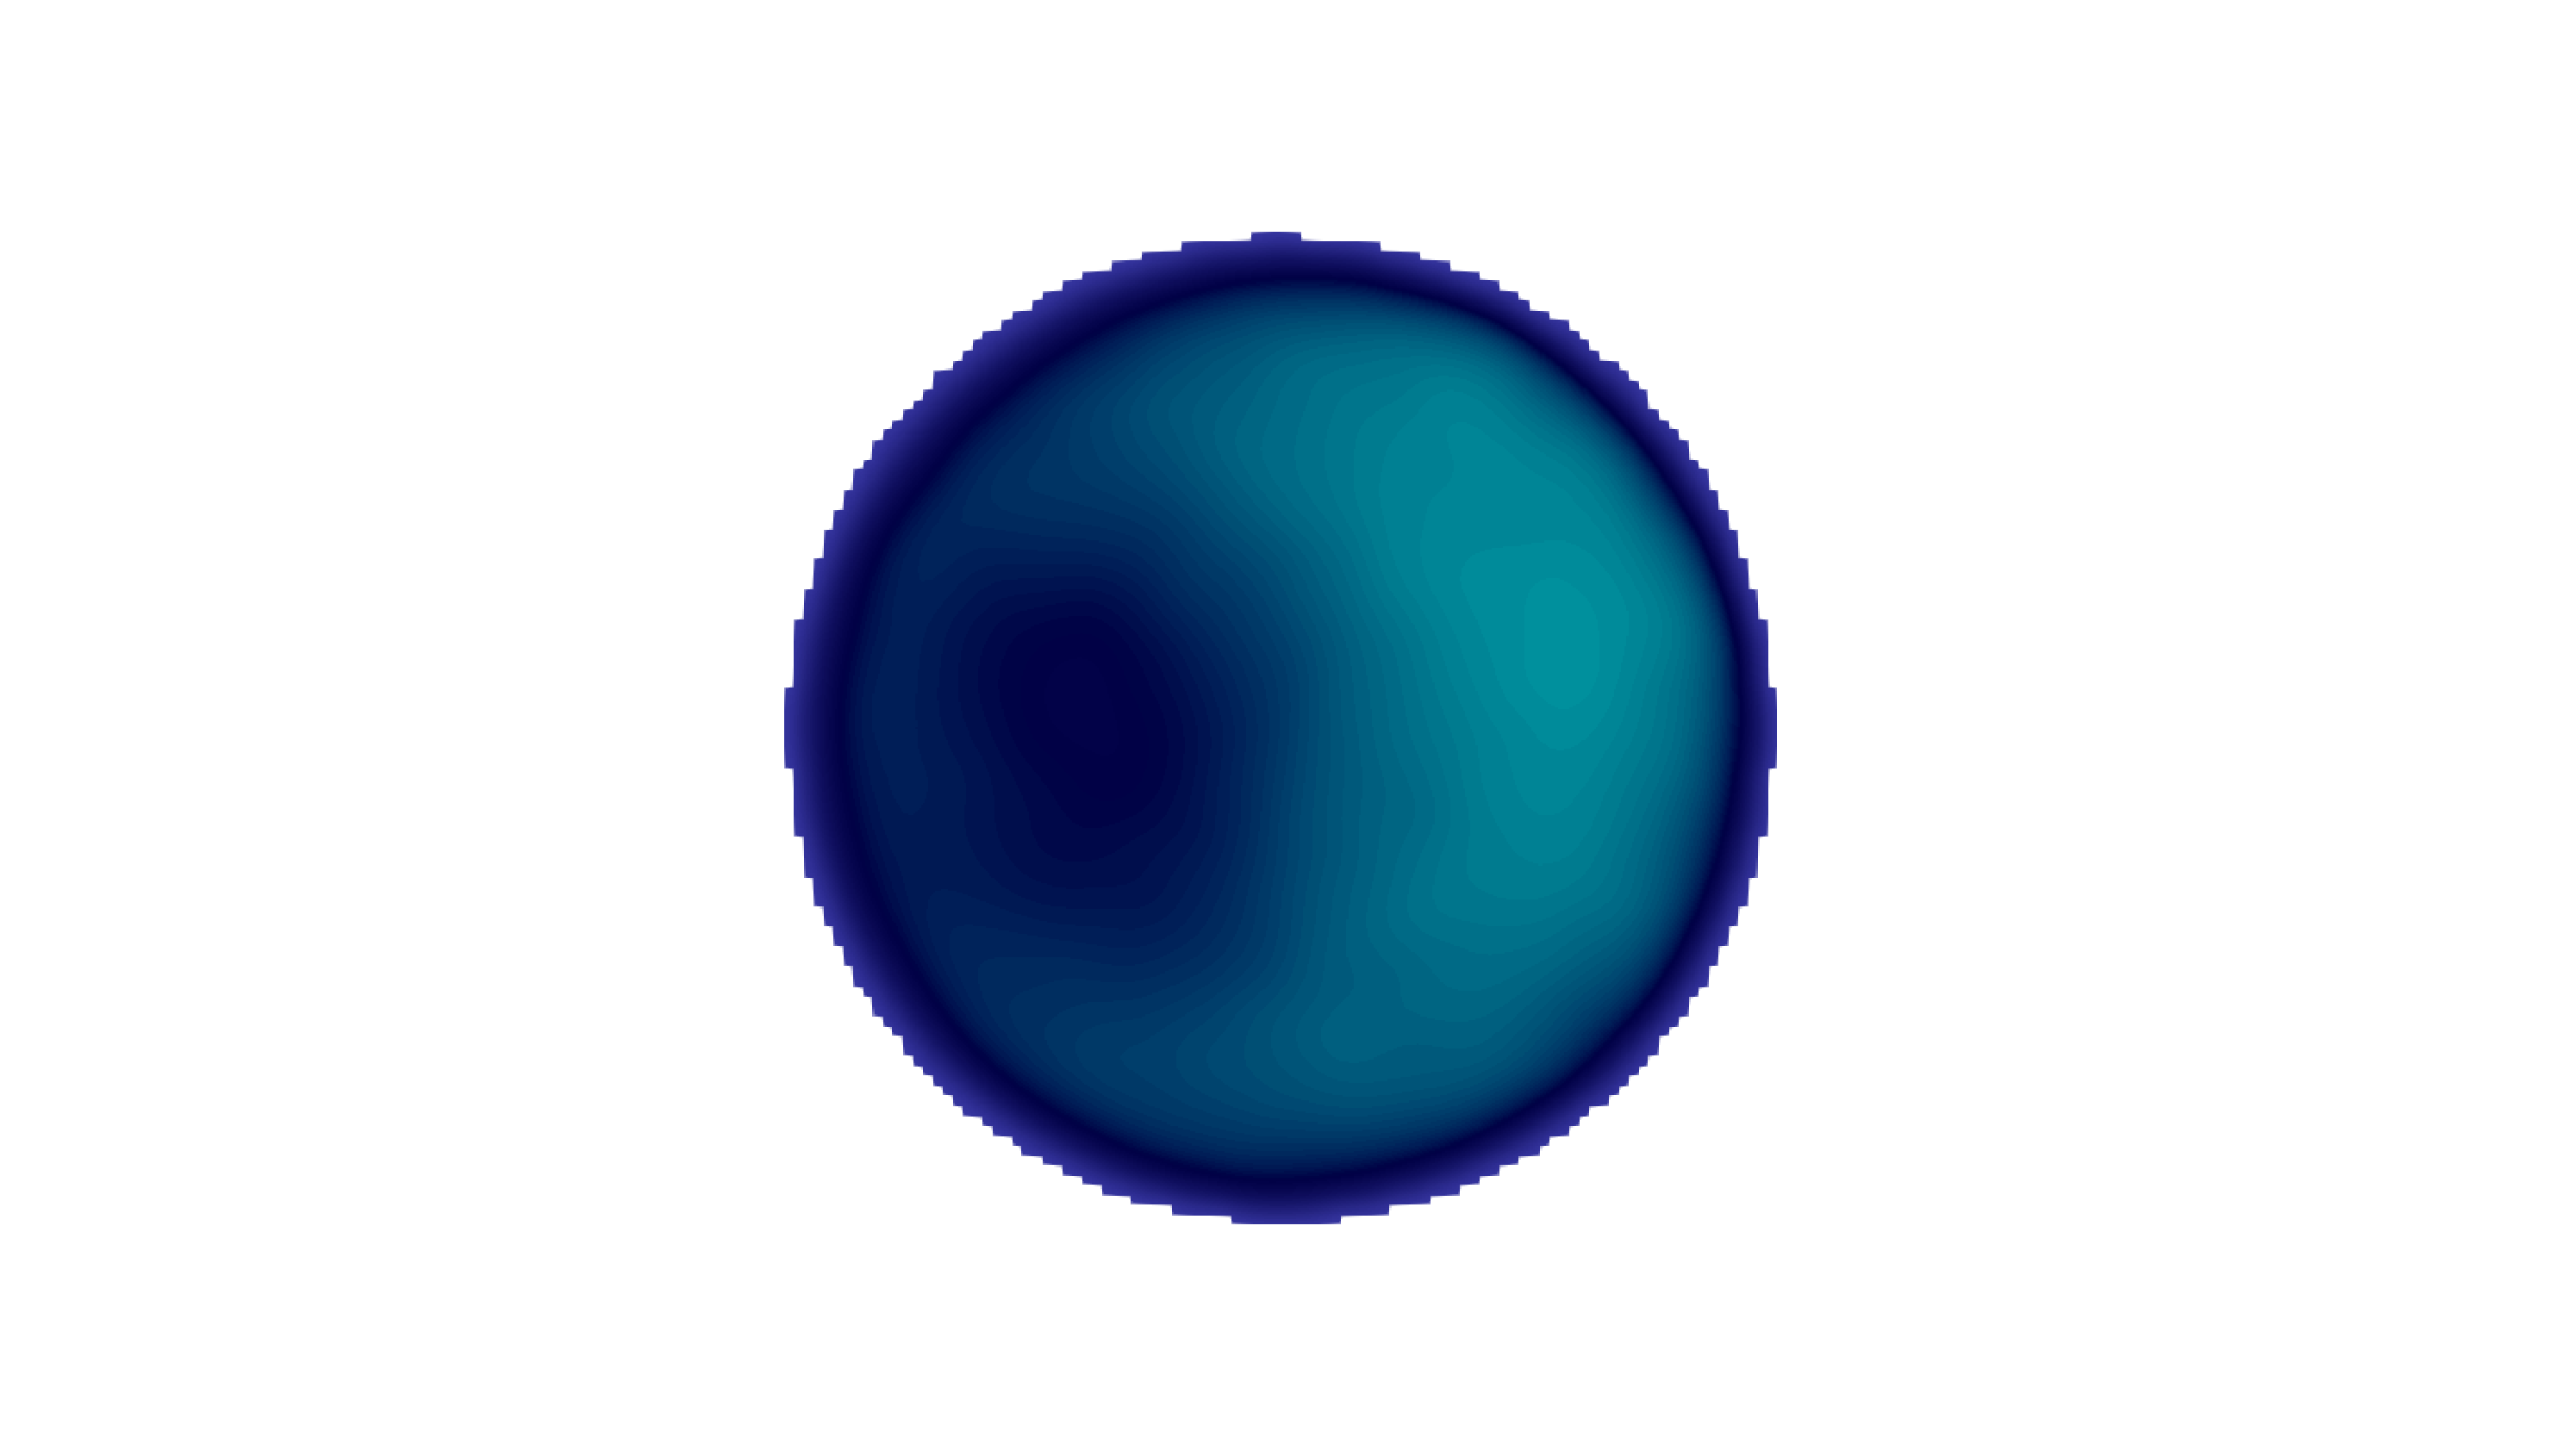
\includegraphics[
		width=0.46\textwidth,
		trim={150mm 20mm 150mm 20mm},
		clip
		]
		{figures/plots/08/08_RPA_mean_veloc.pdf}\\[38pt]
		
		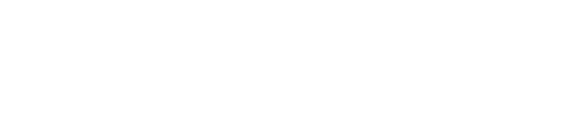
\includegraphics[
		width=1.08\textwidth,
		]
		{figures/plots/filler.pdf}
		\caption{Magnitudes of mean velocity at the outlets \(\Gamma^{\text{LPA}}_{\text{out}}\) and \(\Gamma^{\text{RPA}}_{\text{out}}\).}
		\label{fig:mean_velocity_outlets08}
	\end{subfigure}
	\begin{center}
		\vspace{-30mm}
		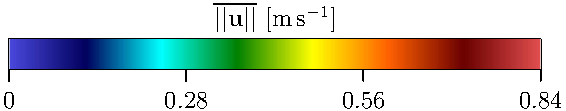
\includegraphics[
		width=0.4\textwidth,
		]
		{figures/plots/mean_veloc_leg.pdf}
		
	\end{center}
	\vspace{14mm}
	
	\begin{subfigure}{0.60\textwidth}
		\centering
		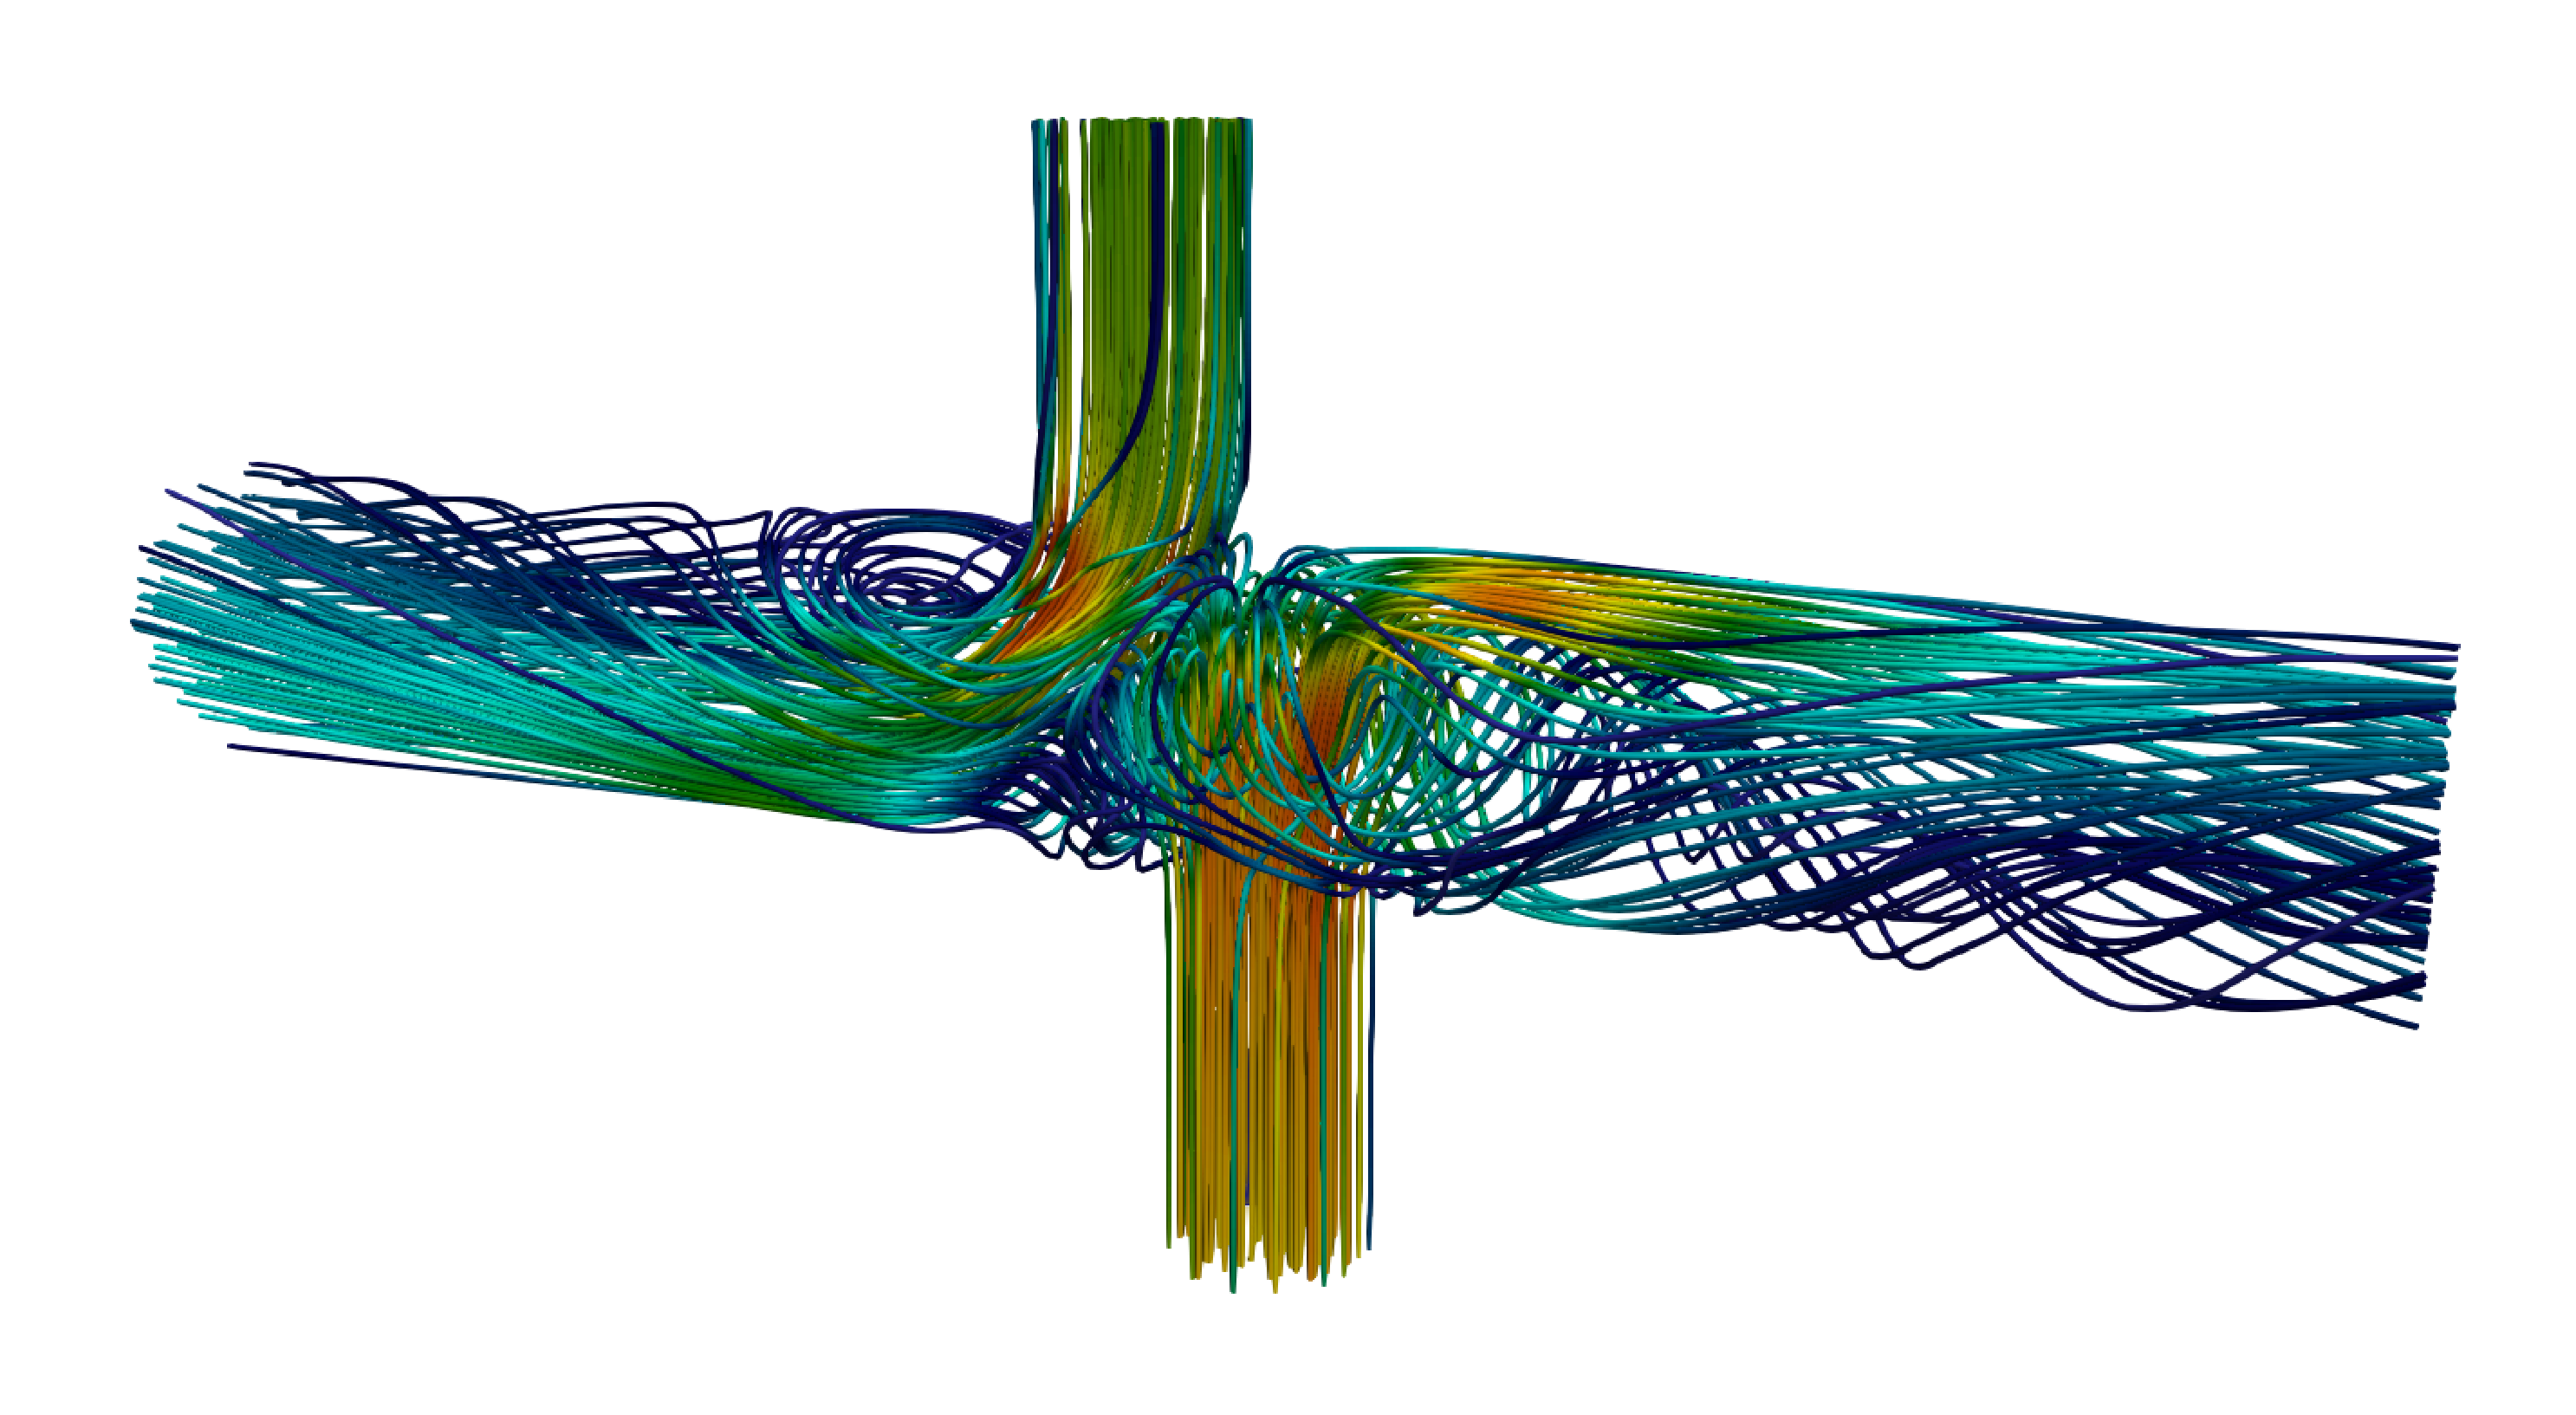
\includegraphics[
		width=\textwidth,
		trim={10mm 10mm 10mm 10mm},
		clip
		]
		{figures/plots/08/08_mean_veloc_streamlines.pdf}%
		\rlap{\hspace{-9cm}\raisebox{0.1cm}{%  move next graphics to top right corner
				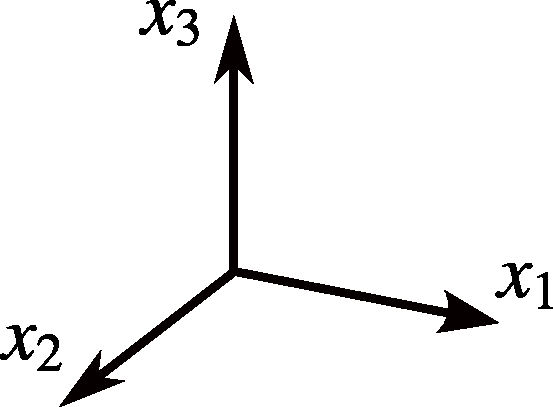
\includegraphics[height=1.5cm]{figures/x1x2x3.pdf}%
		}}
		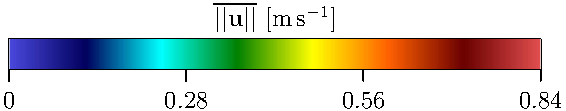
\includegraphics[
		width=0.65\textwidth,
		]
		{figures/plots/mean_veloc_leg.pdf}
		\caption{Streamlines of the mean velocity field illustrating the flow trajectory throughout the geometry.}
		\label{fig:mean_velocity_streamlines08}
	\end{subfigure}\hfill%
	\begin{subfigure}{0.36\textwidth}
		\centering
		\vspace{9mm}
		LPA\hspace{24mm}RPA
		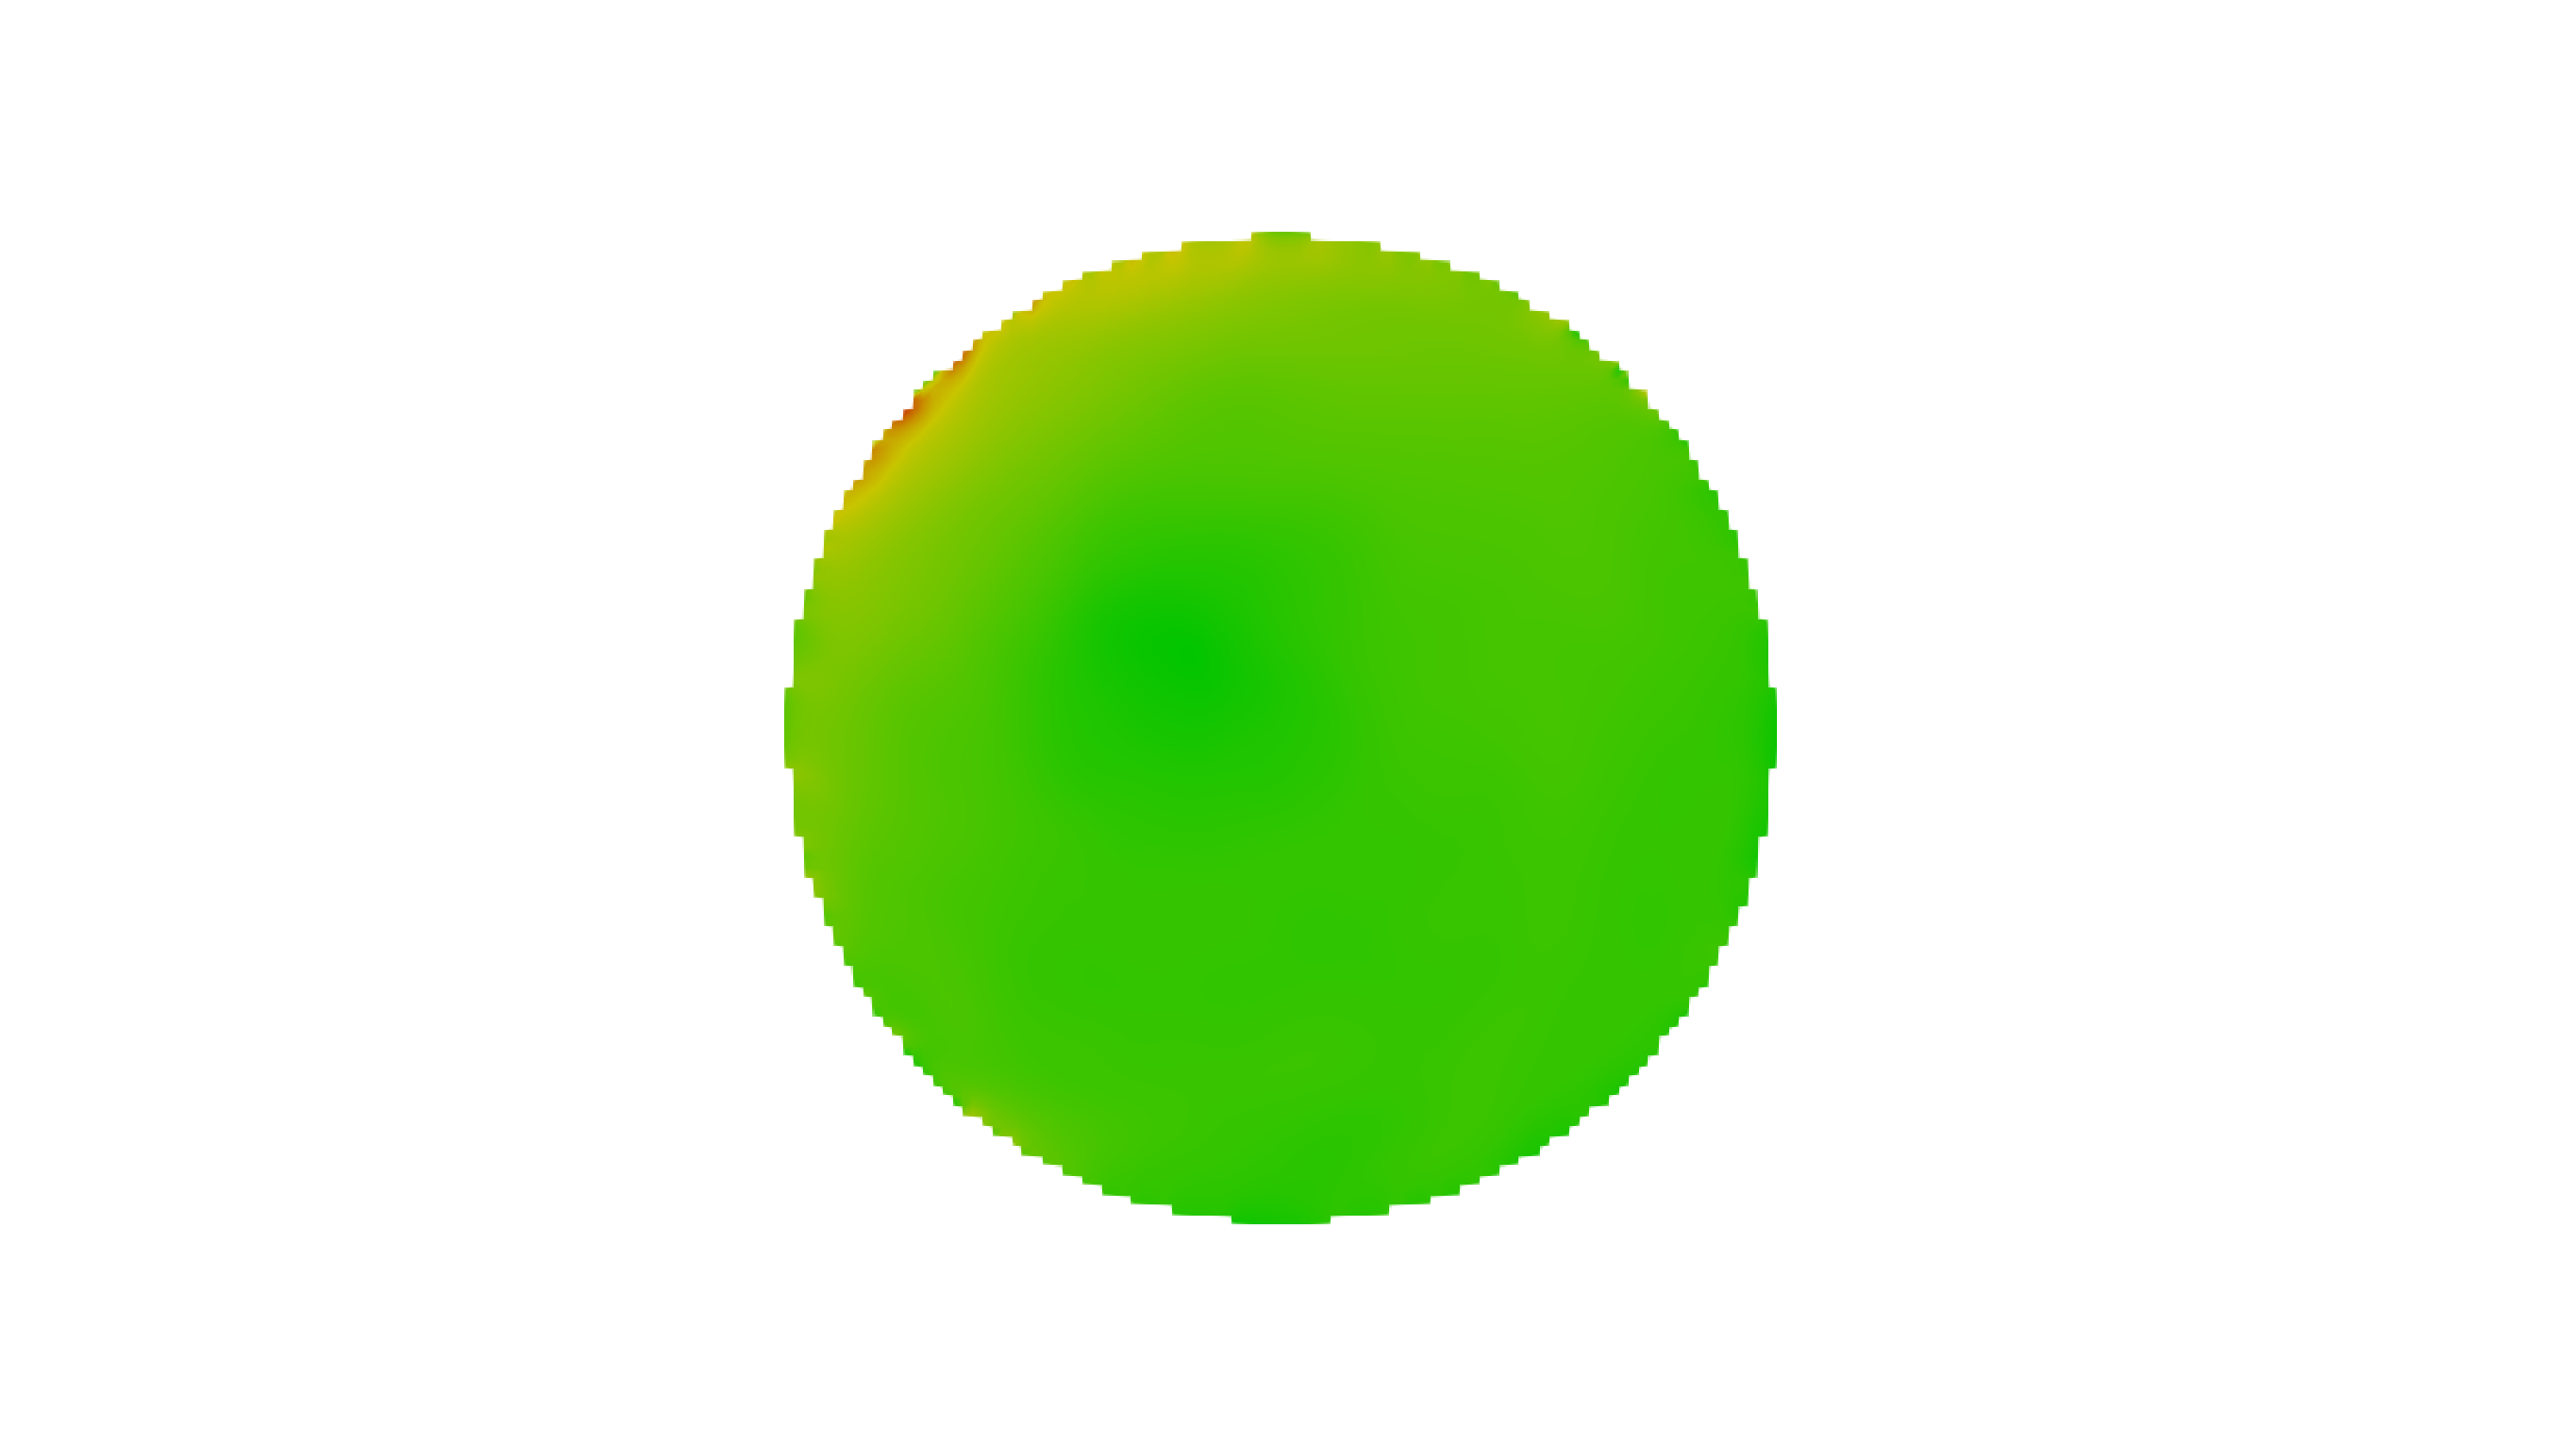
\includegraphics[
		width=0.46\textwidth,
		trim={150mm 20mm 150mm 20mm},
		clip
		]
		{figures/plots/08/08_LPA_angle.pdf}\hfill
		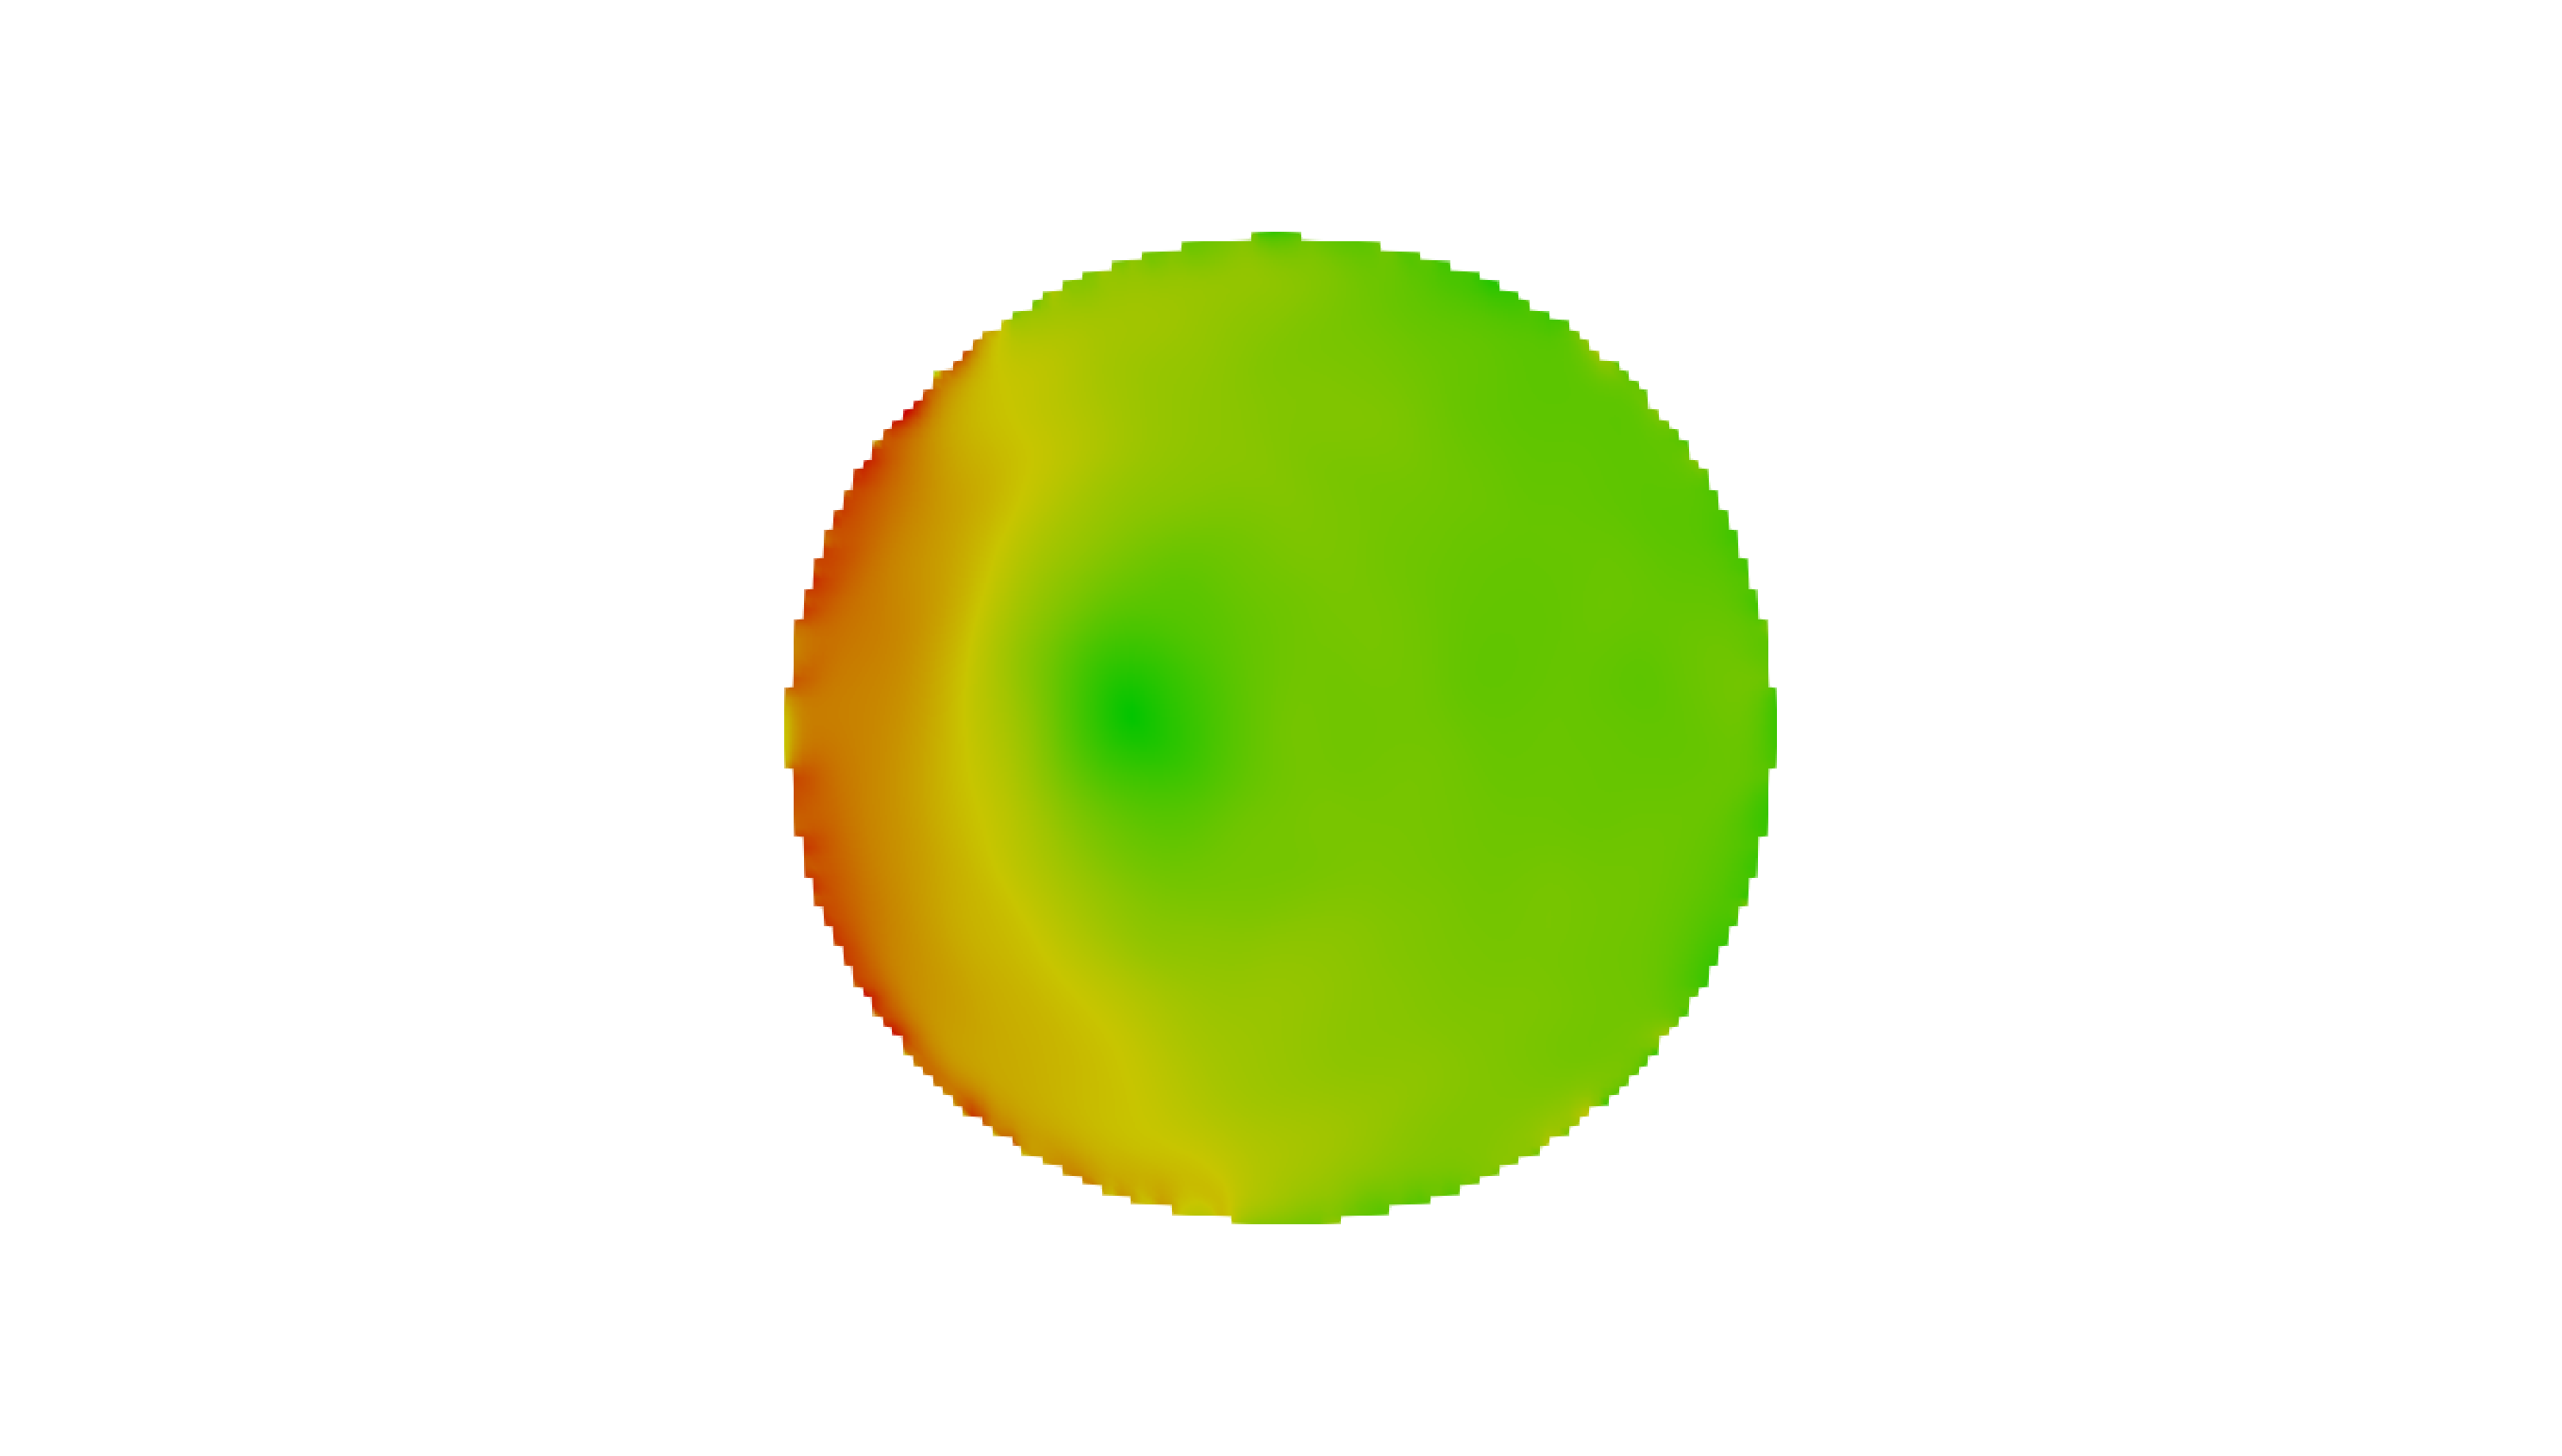
\includegraphics[
		width=0.46\textwidth,
		trim={150mm 20mm 150mm 20mm},
		clip
		]
		{figures/plots/08/08_RPA_angle.pdf}
		
		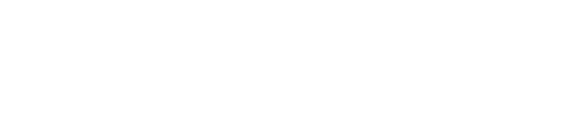
\includegraphics[
		width=0.99\textwidth,
		]
		{figures/plots/filler.pdf}
		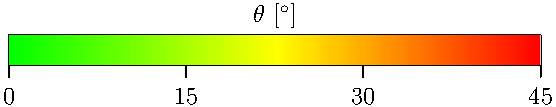
\includegraphics[
		width=1.05\textwidth,
		]
		{figures/plots/angle_leg.pdf}
		\caption{Angle between the mean velocity vector and the normal direction at the outlets \(\Gamma^{\text{LPA}}_{\text{out}}\) and \(\Gamma^{\text{RPA}}_{\text{out}}\).}
		\label{fig:velocity_angle_outlets08}
	\end{subfigure}
	
	\vspace{2mm}
	\caption{Overview of mean velocity fields and outlet characteristics for the case of point P$_8$, i.e., when $o_1 = 0{,}8 \, \mathrm{mm}$. Subfigure (a) shows the velocity magnitude field, (b) displays outlet-specific velocity magnitudes, (c) presents streamlines of the mean velocity field, and (d) details the angular alignment of velocity vectors with outlet normals.}
	\label{fig:mean_velocity_analysis08}
\end{figure}

\newgeometry{top=1.7cm}

\begin{figure}[H]
	\subsection*{Shear rate}
	\vspace{-3mm}
	\rule{\textwidth}{0.4pt}\\
	\begin{subfigure}{0.48\textwidth}
		%		\vspace{-8mm}
		\centering
		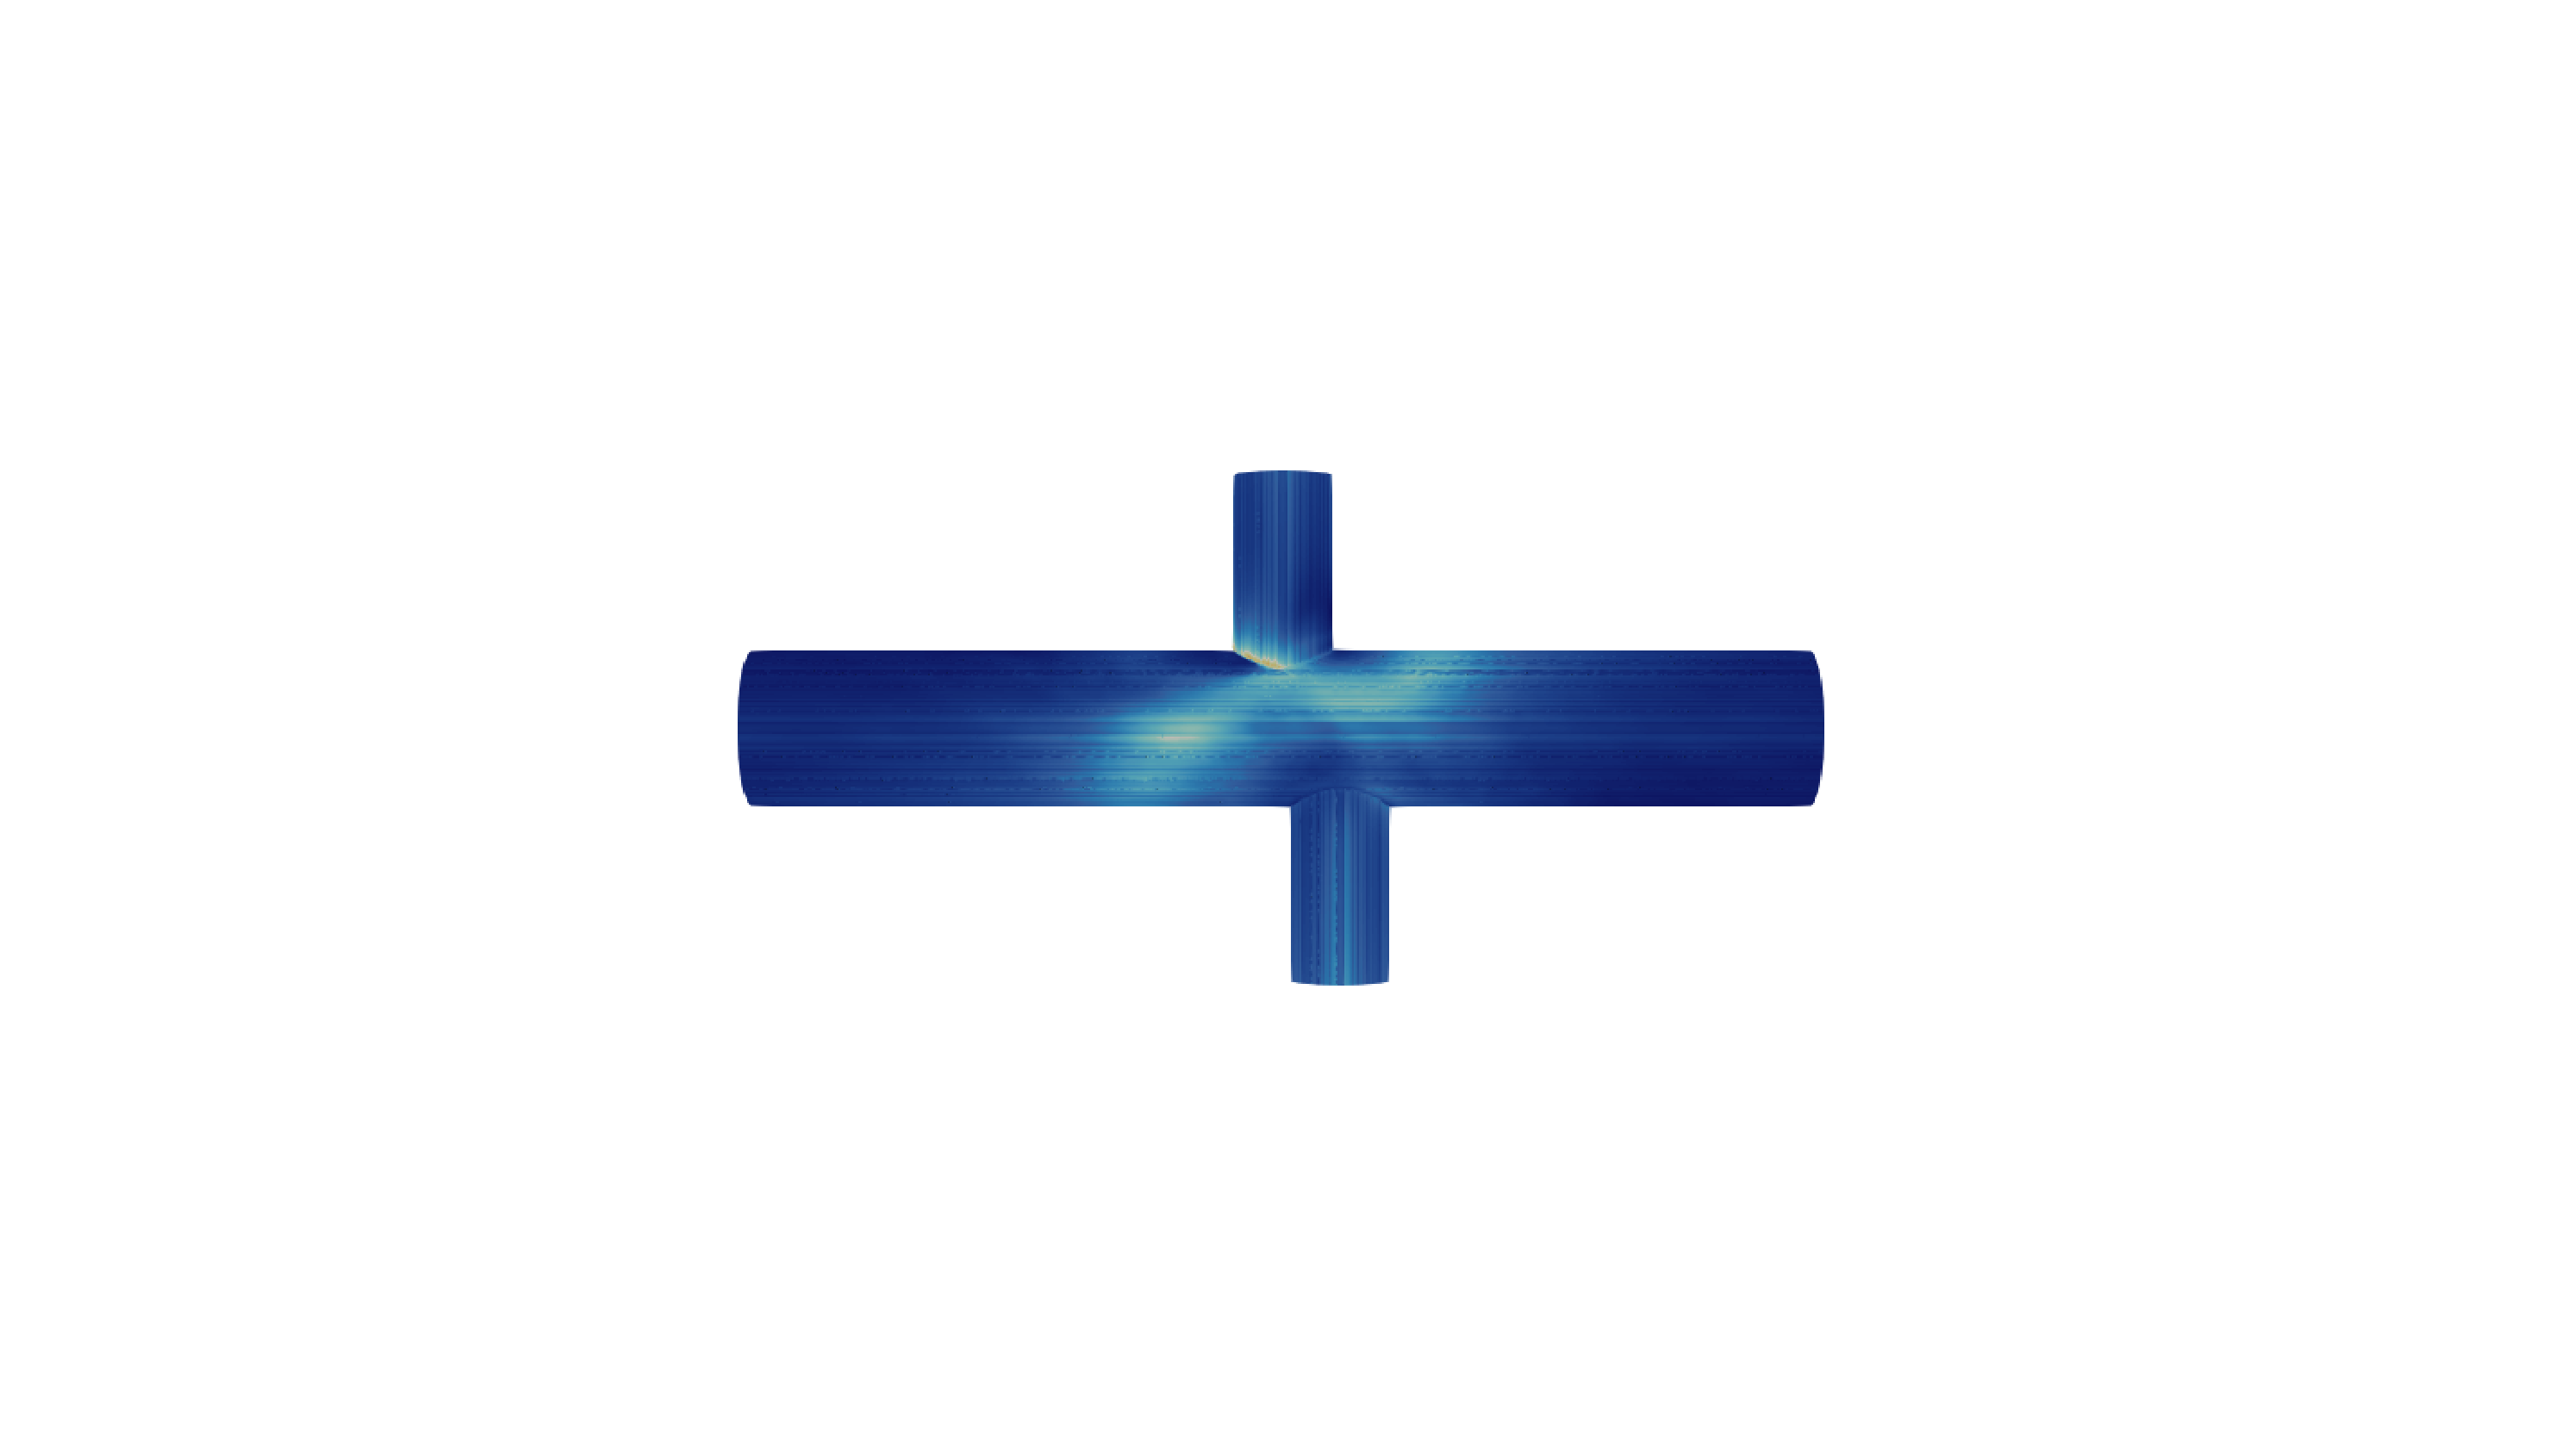
\includegraphics[
		width=\textwidth,
		trim={130mm 85mm 130mm 80mm},
		clip
		]
		{figures/plots/08/08_mean_stress_xz.pdf}%
		\rlap{\hspace{-7cm}\raisebox{-0.5cm}{%  move next graphics to top right corner
				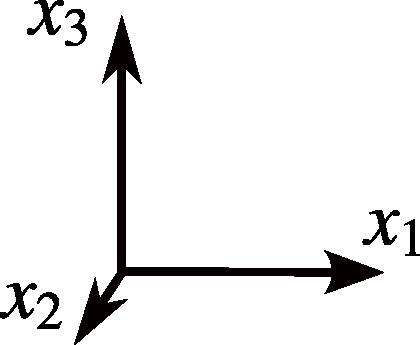
\includegraphics[height=1.5cm]{figures/x1x2x3-side.pdf}%
		}}
		
		
		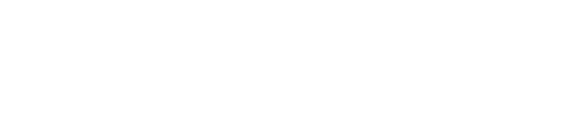
\includegraphics[
		width=0.85\textwidth,
		]
		{figures/plots/filler.pdf}
		\caption{Mean shear rate in the \(x_1\)-\(x_3\) plane.}
		\label{fig:mean_stress_xz08}
		
	\end{subfigure}\hfill%
	\begin{subfigure}{0.48\textwidth}
		%		\vspace{-8mm}
		\centering
		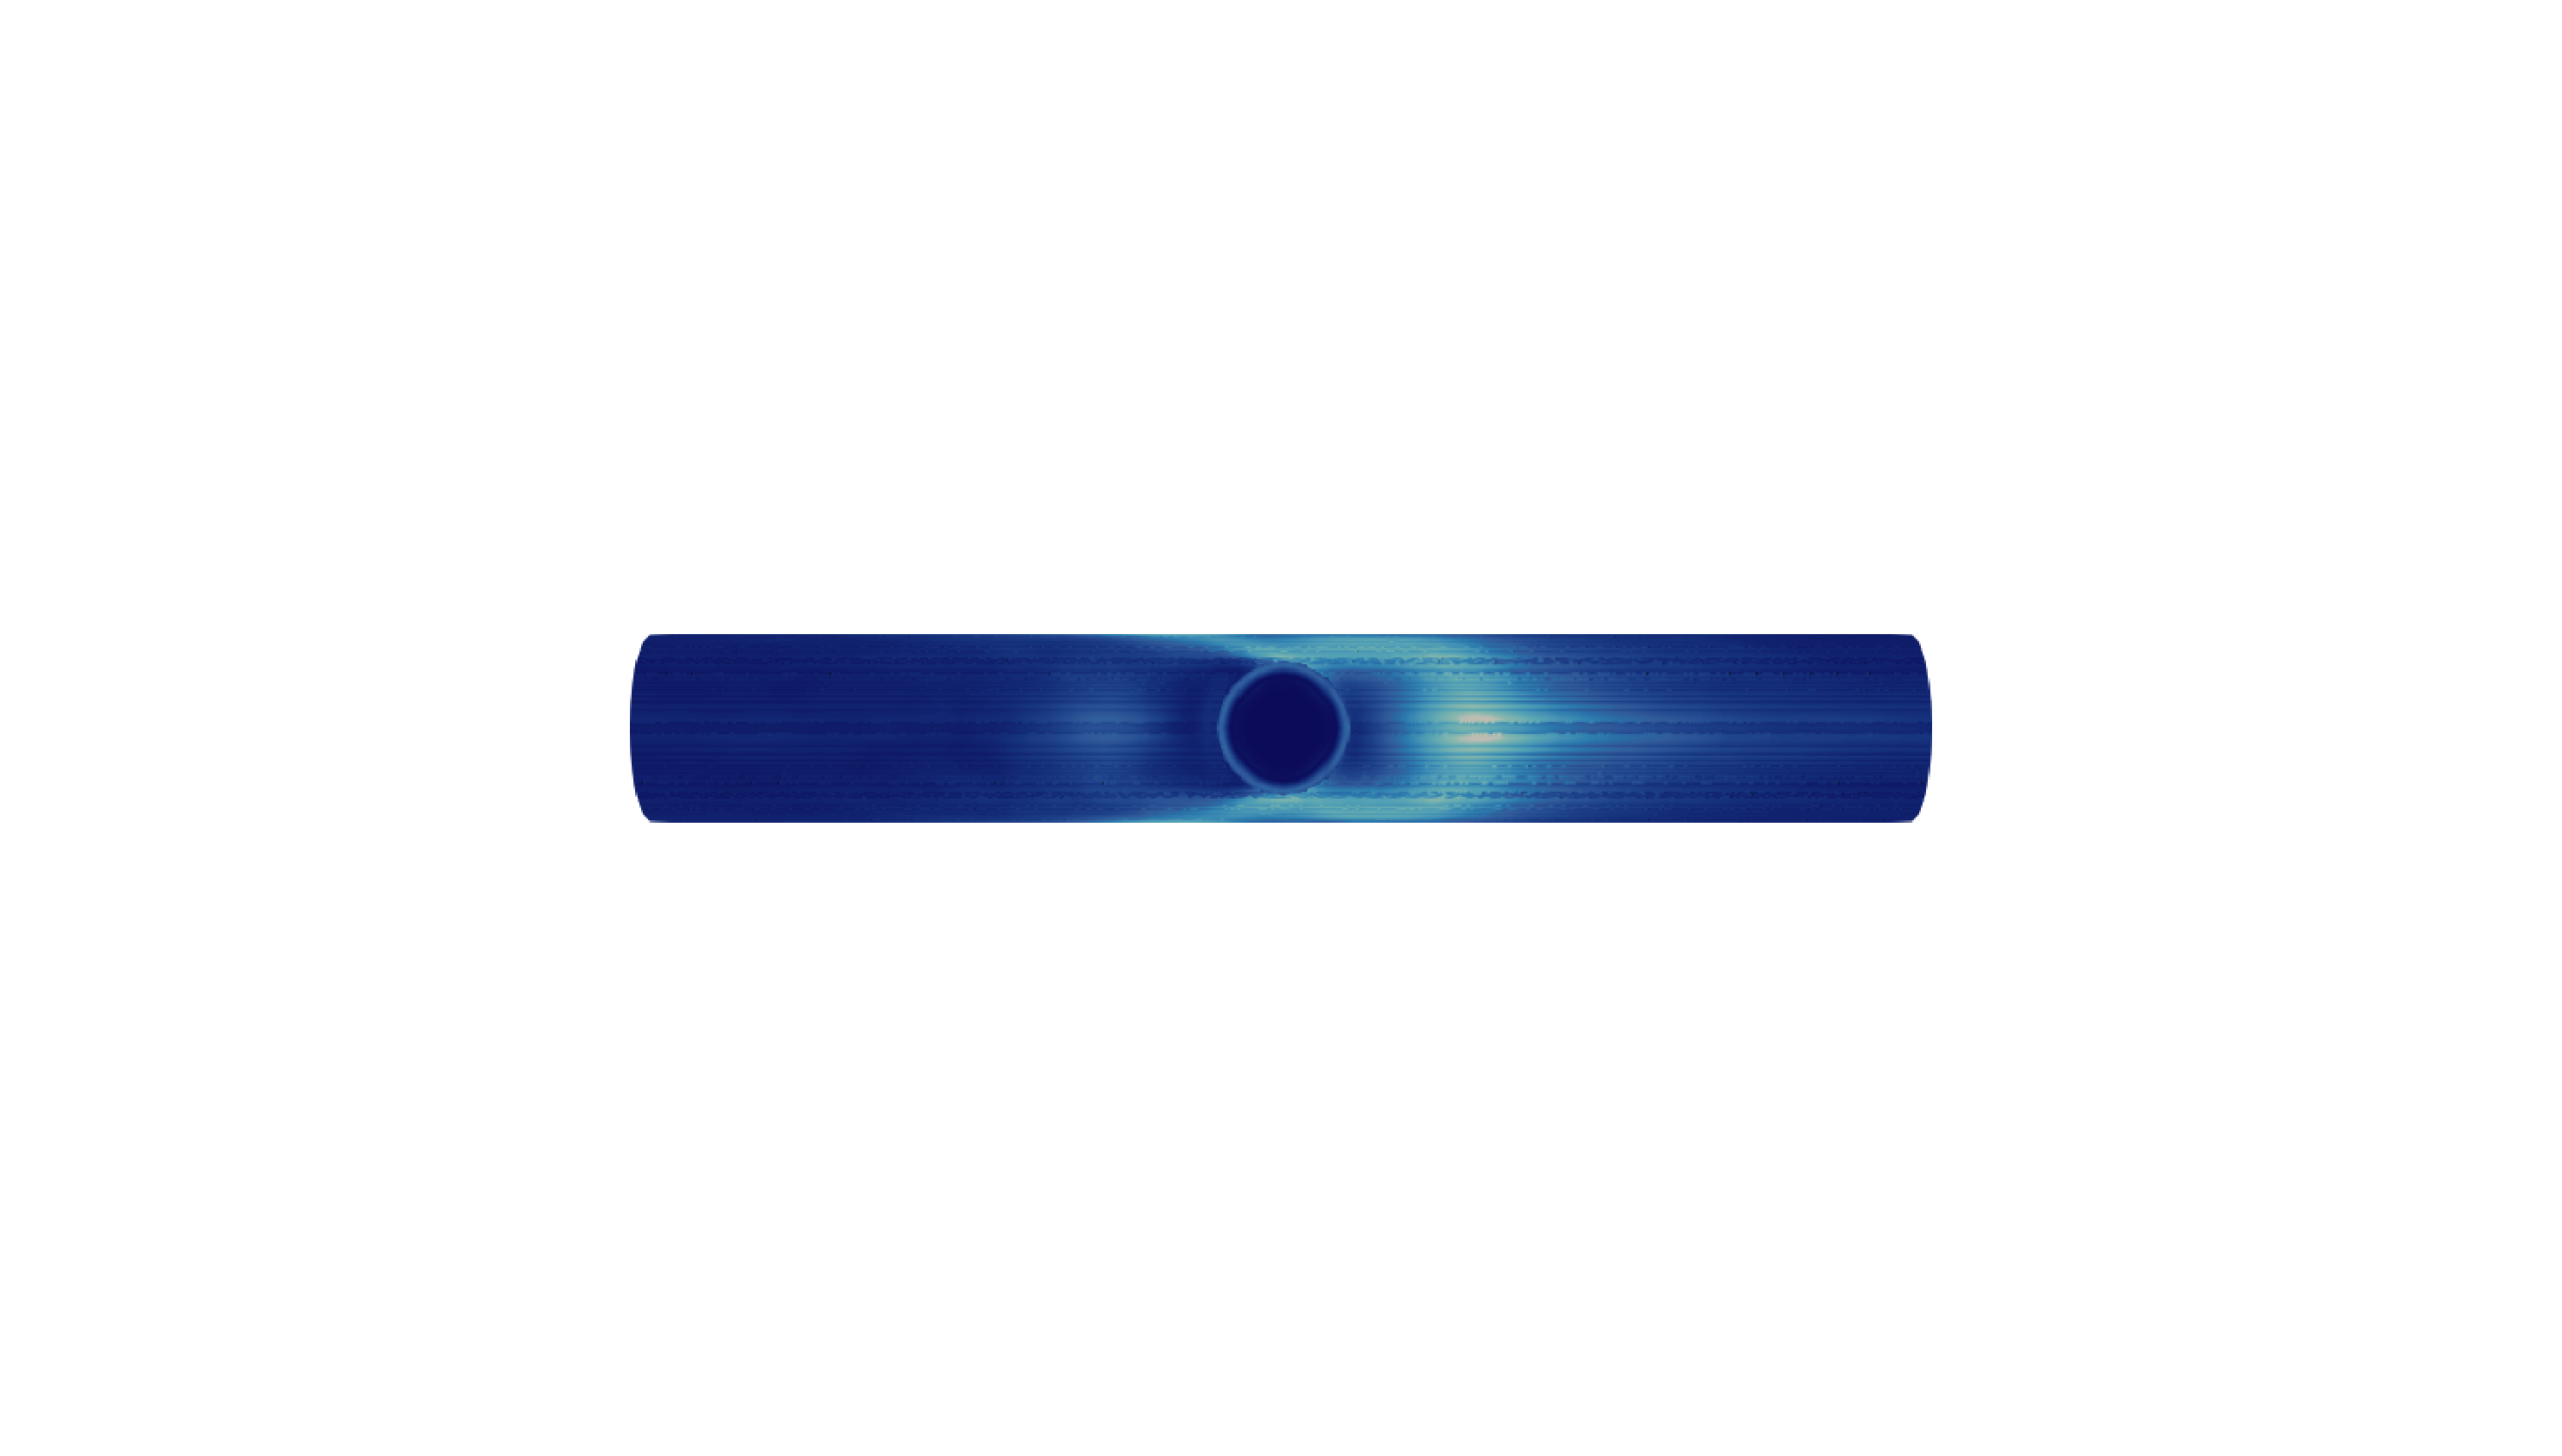
\includegraphics[
		width=\textwidth,
		trim={130mm 85mm 130mm 80mm},
		clip
		]
		{figures/plots/08/08_mean_stress_xy.pdf}%
		\llap{\raisebox{-0.5cm}{%  move next graphics to top right corner
				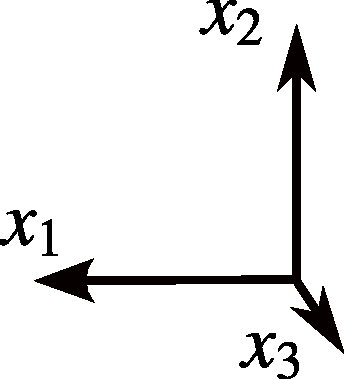
\includegraphics[height=1.5cm]{figures/x1x2x3-top.pdf}%
		}}
		
		
		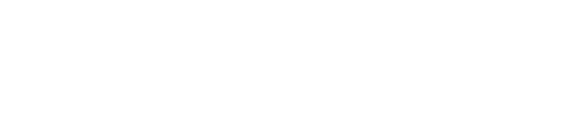
\includegraphics[
		width=0.85\textwidth,
		]
		{figures/plots/filler.pdf}
			\caption{Mean shear rate in the \(x_1\)-\(x_2\) plane.}
		\label{fig:mean_stress_xy08}
	\end{subfigure}
	\begin{center}
		\vspace{-32mm}
		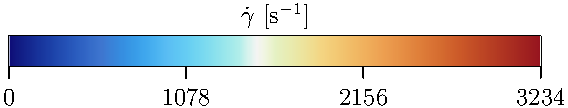
\includegraphics[
		width=0.4\textwidth,
		]
		{figures/plots/mean_stress_leg.pdf}
		
	\end{center}
	
	\vspace{12mm}
    \caption{Mean shear rate visualizations in the \(x_1\)-\(x_3\) and in the \(x_1\)-\(x_2\) plane for the case of point P$_8$, i.e., when $o_1 = 0{,}8 \, \mathrm{mm}$.}
	\label{fig:shear_rate08}
\end{figure}
\vspace{-3mm}
\begin{figure}[H]
	\subsection*{Velocity fluctuations}
	\vspace{-4mm}
	\rule{\textwidth}{0.4pt}\\
	\begin{subfigure}{0.48\textwidth}
%		\vspace{-2mm}
		\centering
		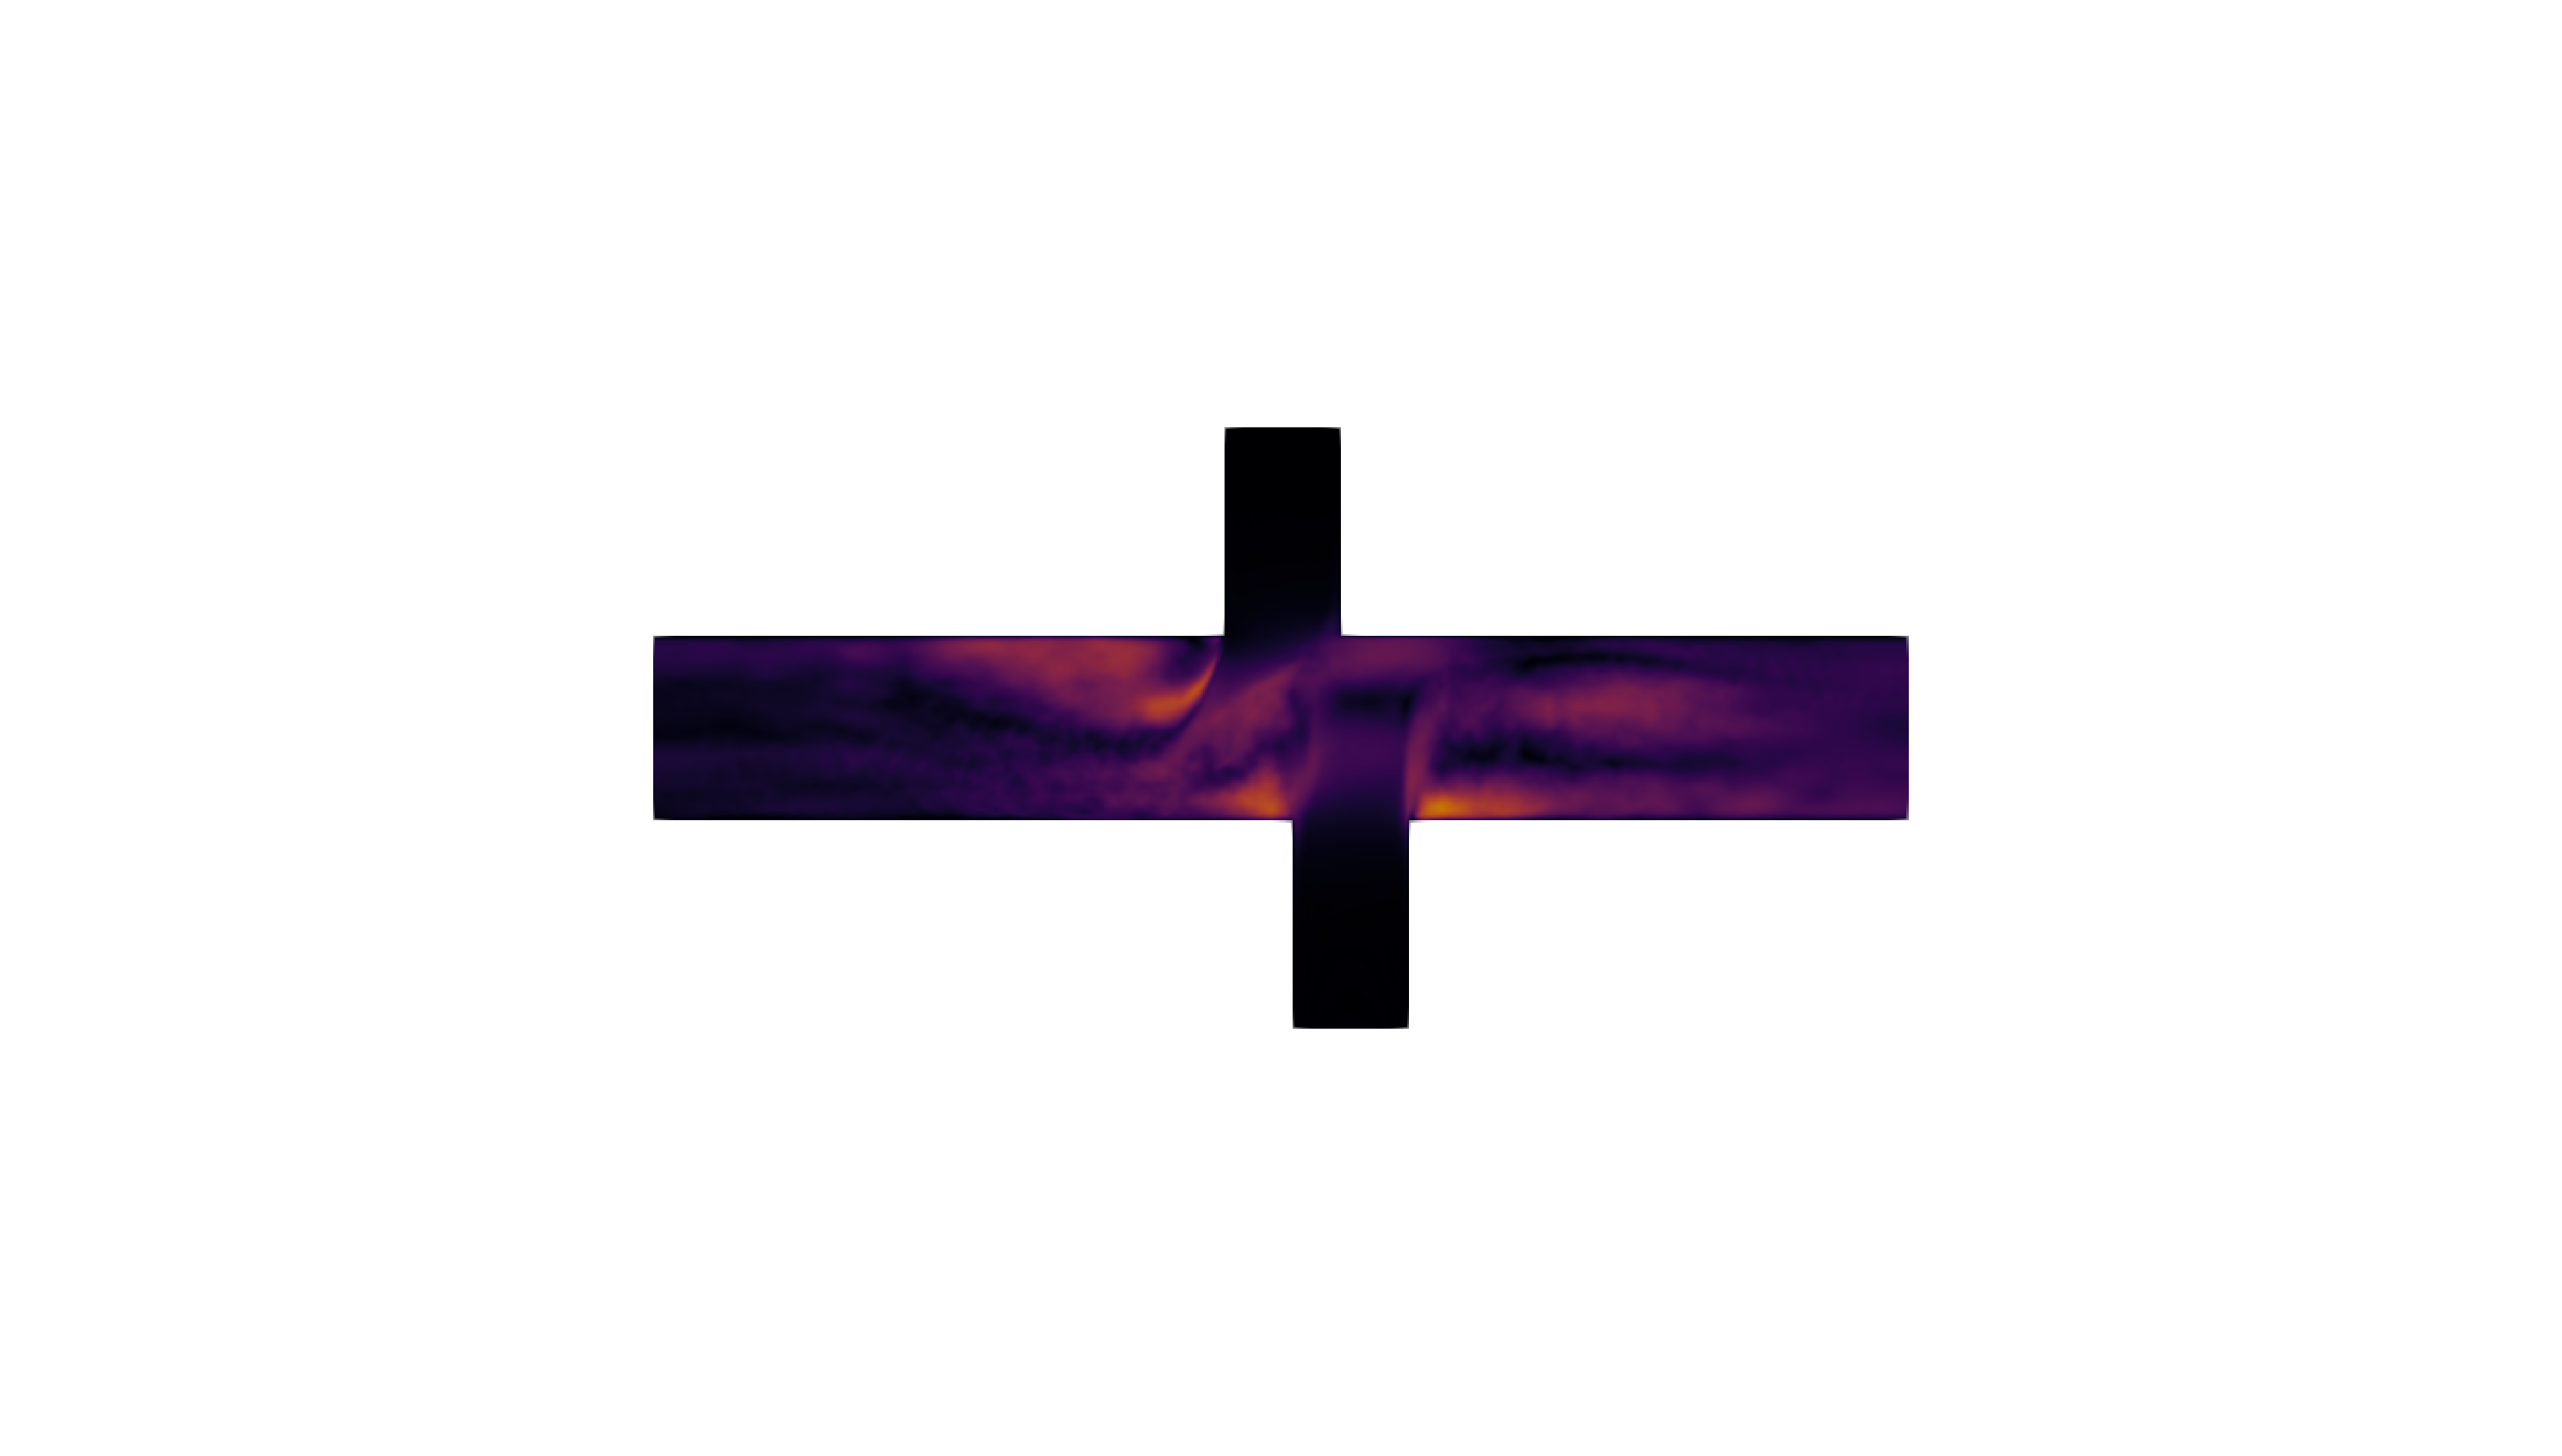
\includegraphics[
		width=\textwidth,
		trim={130mm 85mm 130mm 80mm},
		clip
		]
		{figures/plots/08/08_mean_flucs_xz.pdf}%
		\rlap{\hspace{-7cm}\raisebox{-0.5cm}{%  move next graphics to top right corner
				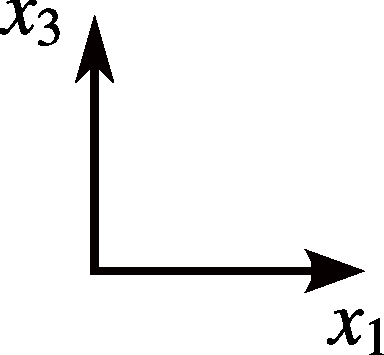
\includegraphics[height=1.5cm]{figures/x1x3.pdf}%
		}}
		
		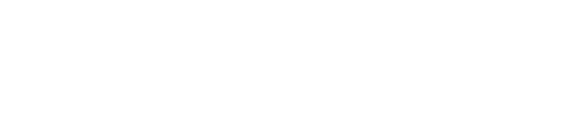
\includegraphics[
		width=0.81\textwidth,
		]
		{figures/plots/filler.pdf}
		\caption{Mean velocity fluctuations magnitude field in the \(x_1\)-\(x_3\) plane.}
		\label{fig:mean_flucs_xz08}
		
	\end{subfigure}\hfill%
	\begin{subfigure}{0.48\textwidth}
		\vspace{-1mm}
		\centering
		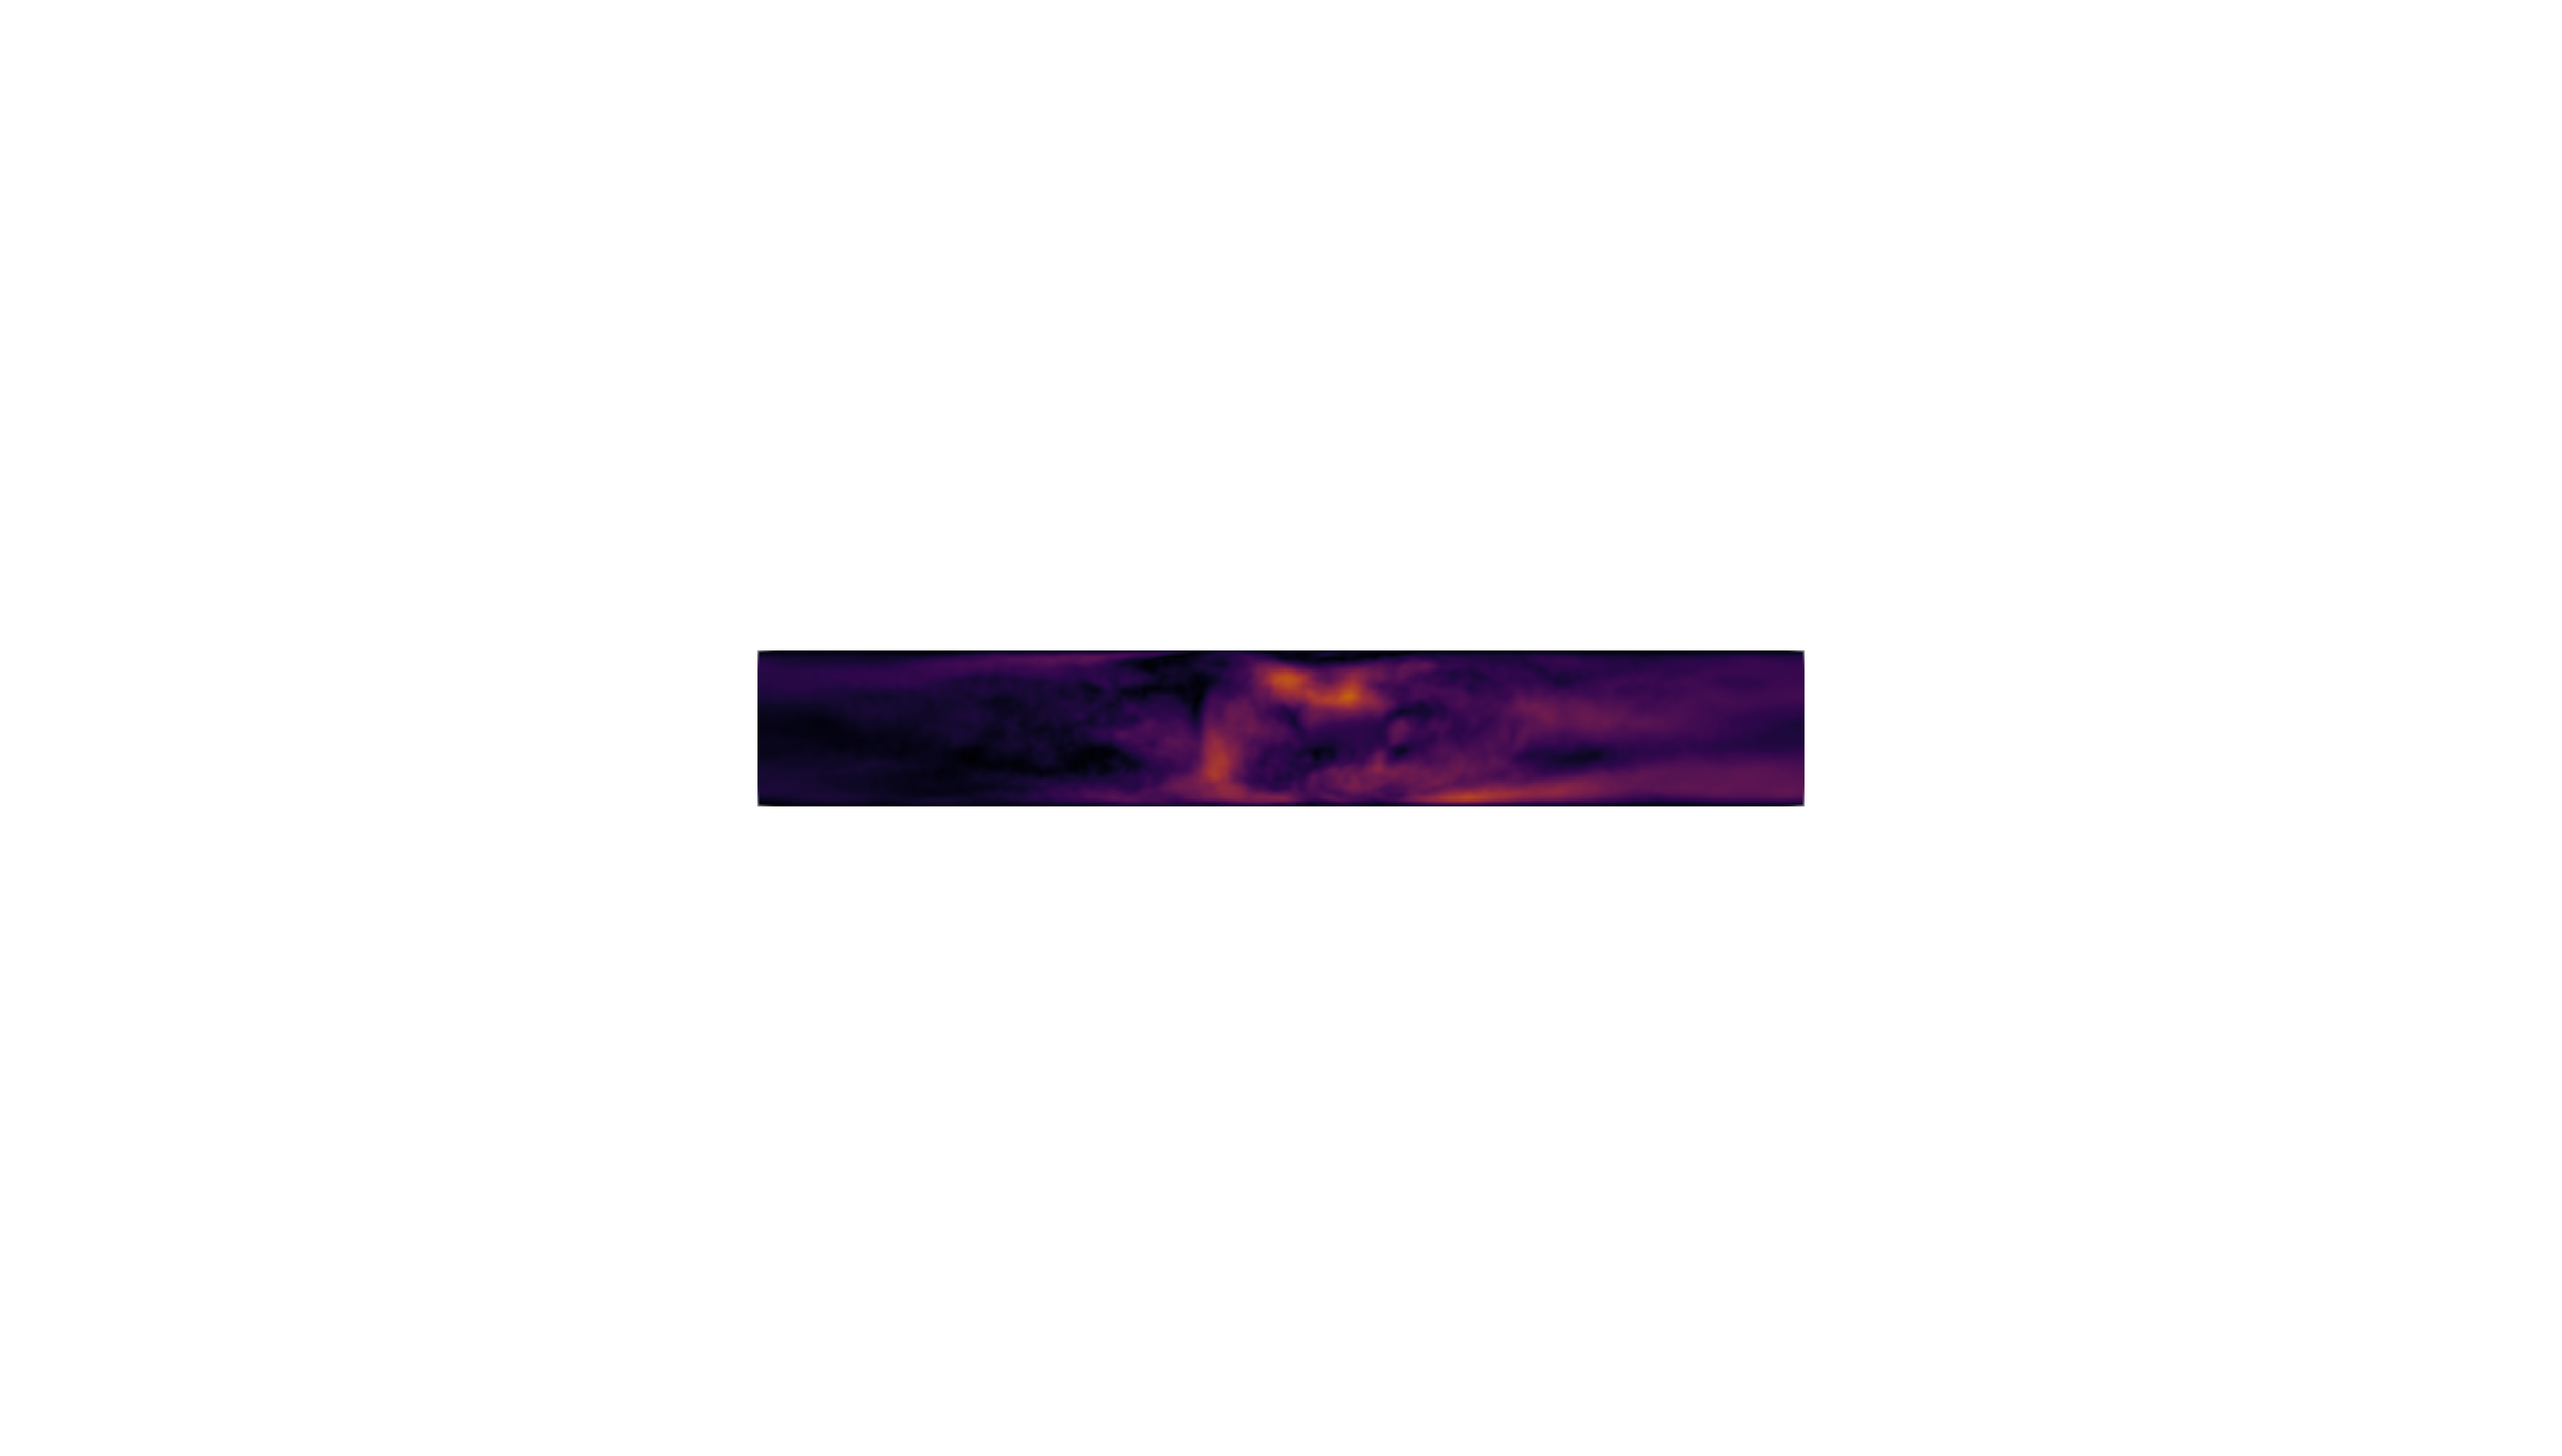
\includegraphics[
		width=1.06\textwidth,
		trim={130mm 98mm 130mm 85mm},
		clip
		]
		{figures/plots/08/08_mean_flucs_xy.pdf}%
		\rlap{\hspace{-1.9cm}\raisebox{-0.7cm}{%  move next graphics to top right corner
				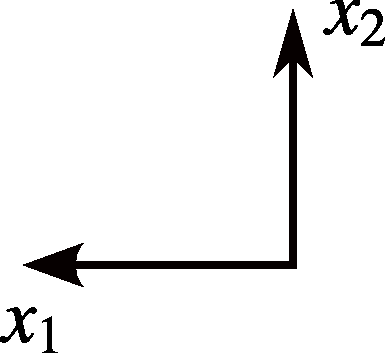
\includegraphics[height=1.5cm]{figures/x1x2.pdf}}}
		
		
		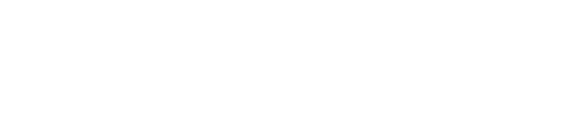
\includegraphics[
		width=0.81\textwidth,
		]
		{figures/plots/filler.pdf}
		\caption{Mean velocity fluctuations magnitude field in the \(x_1\)-\(x_2\) plane.}
		\label{fig:mean_flucs_xy08}
	\end{subfigure}
	\begin{center}
		\vspace{-32mm}
		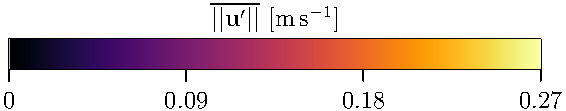
\includegraphics[
		width=0.4\textwidth,
		]
		{figures/plots/mean_flucs_leg.pdf}
		
	\end{center}
	
	\vspace{12mm}
	\caption{Mean velocity fluctuations in the \(x_1\)-\(x_3\) and in the \(x_1\)-\(x_2\) plane for the case when $o_1 = 0{,}8 \, \mathrm{mm}$.}
	\label{fig:velocity_fluctuations08}
\end{figure}
\vspace{-3mm}
\begin{figure}[H]
	\subsection*{SVC/IVC split}
	\vspace{-3mm}
	\rule{\textwidth}{0.4pt}
	\begin{subfigure}{0.60\textwidth}
		\vspace{0mm}
		\centering
		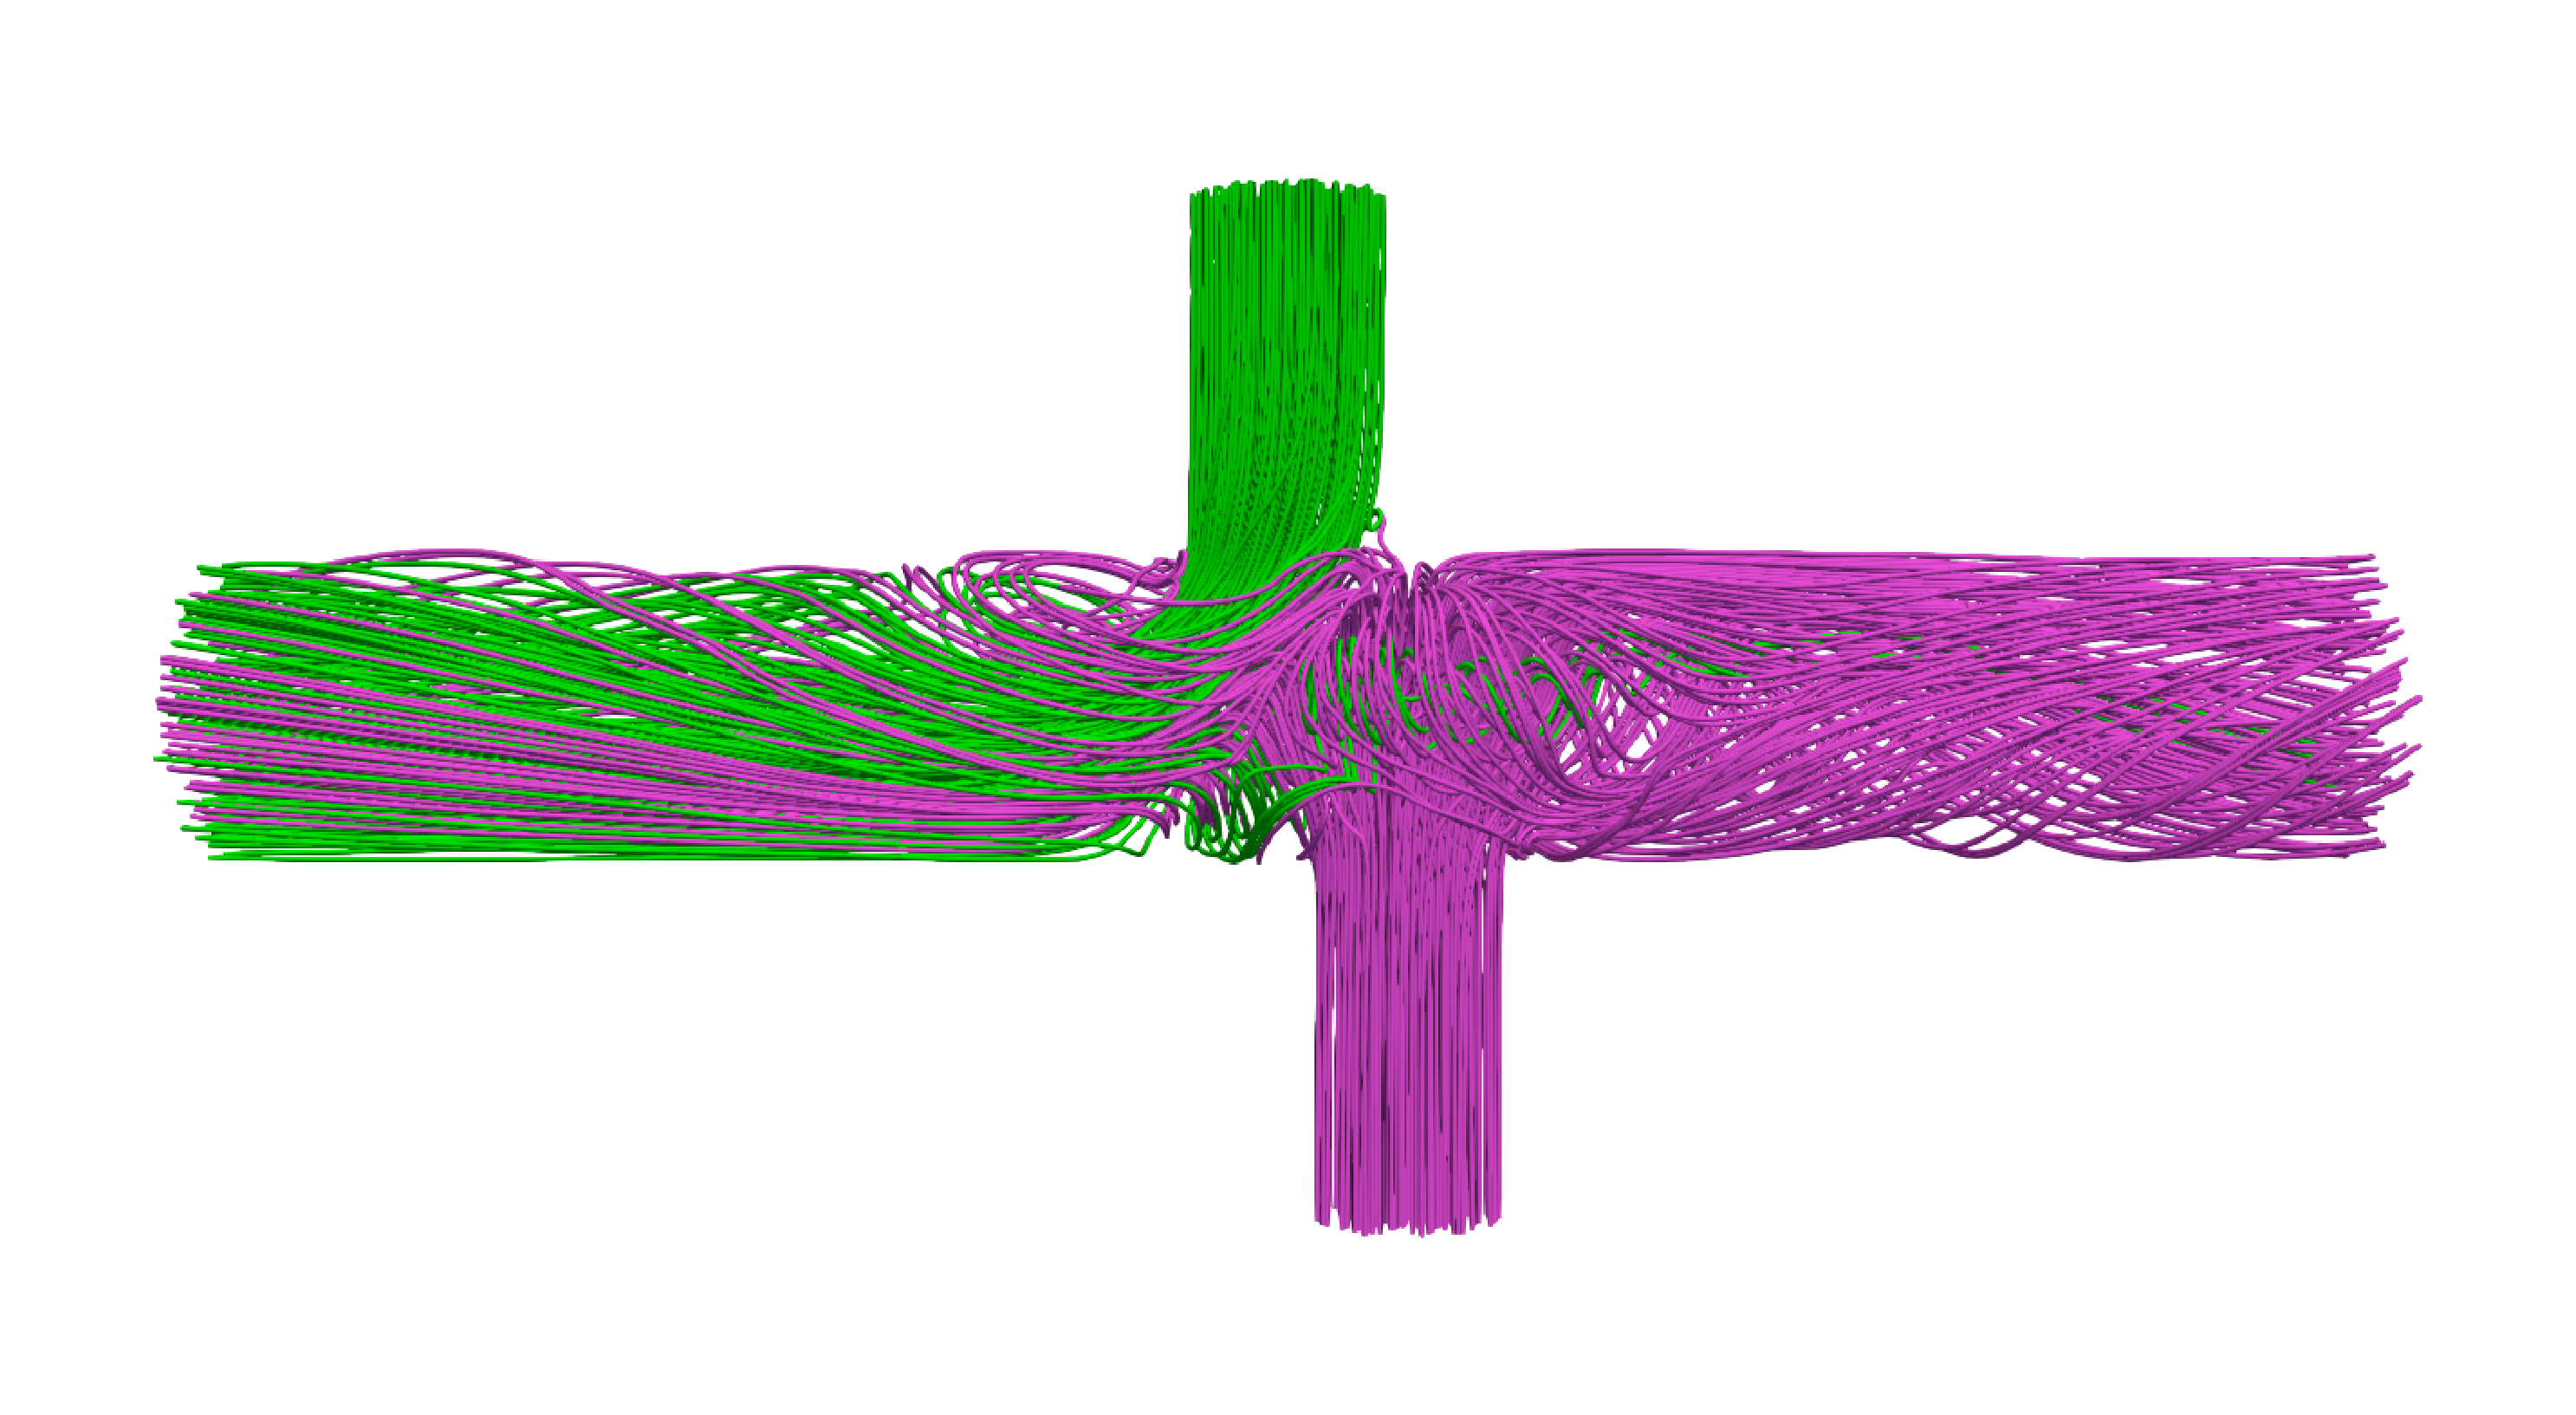
\includegraphics[
		width=\textwidth,
		trim={10mm 10mm 10mm 26mm},
		clip
		]
		{figures/plots/08/08_lpa_rpa_split.pdf}%
		\rlap{\hspace{-8.6cm}\raisebox{-0.0cm}{%  move next graphics to top right corner
				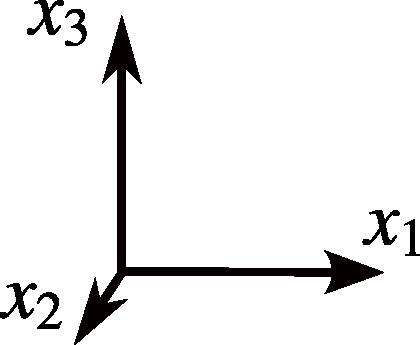
\includegraphics[height=1.5cm]{figures/x1x2x3-side.pdf}%
		}}
		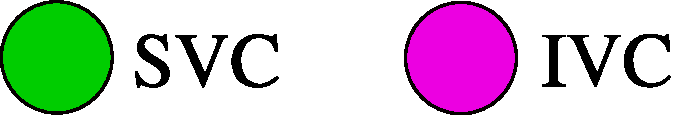
\includegraphics[
		width=0.3\textwidth,
		]
		{figures/plots/split_leg.pdf}
		%			\caption{Placeholder caption.}
	\end{subfigure}\hfill%
	\begin{subfigure}{0.38\textwidth}
		\hspace{7mm}
		\bgroup
		\centering
		\vspace{-0mm}
		\setlength\tabcolsep{3mm}
		\def\arraystretch{1.9}%
		\begin{tabular}{|c|c|c|}
			\hline
			& RPA & LPA \\ \hline
			SVC & 99{,}71\% & 0{,}29\% \\ \hline
			IVC & 23{,}85\% & 76{,}15\% \\ \hline
		\end{tabular}
		%			\caption{Distribution of fluid sources to RPA and LPA.}
		\label{tab:fluid_distribution08}
		\egroup
	\end{subfigure}
	
	\vspace{2mm}
	\caption{Analysis of the split between the SVC and IVC contributions to the LPA and the RPA for the case of point P$_8$, i.e., when $o_1 = 0{,}8 \, \mathrm{mm}$. The figure illustrates the flow split, and the table provides the exact percentages.}
	\label{fig:svc_ivc_split08}
\end{figure}
\vspace{-7mm}
\restoregeometry
\vfill